\chapter{Distance-Based Competitive Task Allocation}
\label{chap:task_allocation}

Chapter~\ref{chap:iapf} established a stable, empirically validated motion-planning controller for
asymmetric dual-arm manipulation, but validated it under a fixed object-to-arm convention, every
detected nut routed to the left arm and every detected bolt to the right
(Section~\ref{sec:iapf_priority}). Chapter~\ref{chap:lit_review} identified this as gap G5: fixed
per-arm object types fail whenever an object appears outside its designated arm's zone, market-based
methods incur centralized bidding bottlenecks, round-robin ignores spatial conflict, and
learning-based allocation requires extensive offline training while excluding physical task
locations from its state representation~\citep{sk2025competitive}.

This chapter presents a distance-based competitive task allocation mechanism that closes gap G5,
replacing the fixed nut/bolt convention with a temporal proposal window that lets either arm claim
whichever detected object it is actually closest to, regardless of type. The iAPF controller of
Chapter~\ref{chap:iapf}, Equations~\eqref{eq:iapf_attract}--\eqref{eq:iapf_angular}, is reused here
entirely unchanged as the execution layer: once an object is assigned to an arm, that arm still
reaches it under the same three-way equilibrium and the same priority-lock critical-state switching
validated in Section~\ref{sec:iapf_validation}. What changes is only
the question the fixed convention answered by assumption: which arm should handle a given detected
object. Section~\ref{sec:cta_allocation} develops the allocation mechanism itself,
Section~\ref{sec:cta_tuning} refines the force scaling supporting it, and
Section~\ref{sec:cta_results} presents its experimental validation.

%% ============================================================
\section{Distance-Based Competitive Task Allocation}\label{sec:cta_allocation}
%% ============================================================

Rather than assigning each arm a fixed object type, the allocation mechanism lets each idle arm
evaluate incoming detections and commit to the closest reachable one, while resolving conflicts
between the two arms and giving each arm a short window to reconsider before committing.

%% ------------------------------------------------------------
\subsection{Proximity-Based Selection and Reachability}\label{subsec:cta_proximity}
%% ------------------------------------------------------------

For each object type $\tau \in \{\text{nut}, \text{bolt}\}$ and each idle arm $\alpha \in \{L, R\}$,
the system selects the closest detected object of that type to the arm's current end-effector
position:
\begin{equation}
i^*, p^*, d^* = \arg\min_{i \in O_\tau} \left\lVert p_{ee}^\alpha - p^{B_L}_i \right\rVert_2,
\label{eq:cta_selection}
\end{equation}
where $O_\tau$ is the set of currently detected objects of type $\tau$ and $p_i^{B_L}$ is object
$i$'s position from Section~\ref{sec:iapf_architecture}. A candidate object must also satisfy a
reachability constraint before it can be proposed:
\begin{equation}
\psi(\alpha, p) =
\begin{cases}
1, & \lVert p - p_{\text{origin}}^\alpha \rVert_2 < 0.5\,\text{m}, \\
0, & \text{otherwise},
\end{cases}
\label{eq:cta_reachability}
\end{equation}
where $p_{\text{origin}}^\alpha$ is arm $\alpha$'s base origin, restricting proposals to a $0.5$\,m
workspace radius, the same reachability-style test used in Equation~\eqref{eq:sv_reach}, though here
a circular rather than axis-aligned box constraint.

%% ------------------------------------------------------------
\subsection{Spatial Conflict Resolution and Target Management}\label{subsec:cta_conflict}
%% ------------------------------------------------------------

To prevent both arms from committing to the same physical object, a spatial conflict test compares a
new candidate against every already-assigned target:
\begin{equation}
\phi(\tau, \alpha, p) =
\begin{cases}
1, & \exists\, p_{\text{prev}} : \tau_{\text{prev}} = \tau \text{ and } \lVert p_{\text{prev}} - p \rVert_2 < 0.01\,\text{m}, \\
0, & \text{otherwise},
\end{cases}
\label{eq:cta_conflict}
\end{equation}
flagging a conflict whenever a previously assigned target of the same type lies within $0.01$\,m of
the candidate, close enough that the two detections almost certainly refer to the same physical
object rather than two distinct ones. Each arm maintains a target store holding the best proposal
seen so far in the current evaluation window,
\begin{equation}
S_\alpha = (d^*, O^*) \text{ or } \varnothing,
\label{eq:cta_store}
\end{equation}
and a new proposal replaces the stored target according to a competitive update rule that favours
the new candidate unless the stored one is already meaningfully closer:
\begin{equation}
\gamma_{\text{upd}}(d_{\text{new}}, d_{\text{prev}}) =
\begin{cases}
1, & d_{\text{prev}} > d_{\text{new}} - 0.005\,\text{m} \text{ and proposals} < 5, \\
0, & \text{otherwise}.
\end{cases}
\label{eq:cta_update}
\end{equation}
The $0.005$\,m margin prevents the store from oscillating between two nearly equidistant objects,
and the five-proposal cap bounds how long an arm can keep looking before it must act.

%% ------------------------------------------------------------
\subsection{Task Execution and Reset Protocol}\label{subsec:cta_execution}
%% ------------------------------------------------------------

Once its proposal window is exhausted, an arm executes on whatever target its store holds under the
iAPF controller of Chapter~\ref{chap:iapf}, or waits if none was found:
\begin{equation}
E_\alpha =
\begin{cases}
\text{execute}(p_{\text{pick}}, p_{\text{drop}}), & S_\alpha \neq \varnothing, \\
\text{wait}, & \text{otherwise},
\end{cases}
\label{eq:cta_execution}
\end{equation}
with the drop location fixed by object type to sort bolts and nuts into separate bins, exactly as
in the original fixed-assignment validation, only now the \emph{picking} arm is decided
competitively rather than by object type:
\begin{equation}
p_{\text{drop}} =
\begin{cases}
[0, -180, 90]^\top, & \tau = \text{bolt}, \\
[0, -180, 270]^\top, & \tau = \text{nut},
\end{cases}
\label{eq:cta_dropzone}
\end{equation}
after which every per-arm counter and store resets, $n_\alpha \leftarrow 0$,
$\beta_\alpha \leftarrow \text{true}$, $S_\alpha \leftarrow \varnothing$, and the arm becomes
eligible for a fresh evaluation window. Algorithm~\ref{alg:cta_temporal} summarizes the complete
temporal proposal window mechanism, which achieves $\mathcal{O}(n_{\max} \cdot |O|)$ complexity for
proposal window size $n_{\max} = 5$ and detected object count $|O|$, well within the budget of the
30\,FPS detection and 10\,Hz control loop.

\begin{algorithm}[htbp]
\caption{Temporal Proposal Window Mechanism}
\label{alg:cta_temporal}
\begin{algorithmic}[1]
\STATE \textbf{Init:} $n_\alpha \leftarrow 0$, $\beta_\alpha \leftarrow \text{true}$, $S_\alpha \leftarrow \varnothing$
\FOR{each detection $(i, \tau, p, \text{size})$ with arm $\alpha$ idle}
    \STATE $(d^*, p^*) \leftarrow$ closest object of type $\tau$ by Equation~\eqref{eq:cta_selection}
    \IF{$\psi(\alpha, p^*) = 1$ and $\phi(\tau, \alpha, p^*) = 0$}
        \IF{$n_\alpha < 5$}
            \IF{$S_\alpha = \varnothing$ or $\gamma_{\text{upd}}(d^*, d_{\text{prev}}) = 1$}
                \STATE $S_\alpha \leftarrow (d^*, \text{Object}(\tau, \text{size}, p^*))$
            \ENDIF
            \STATE $n_\alpha \leftarrow n_\alpha + 1$
        \ELSE
            \STATE $\beta_\alpha \leftarrow \text{false}$
        \ENDIF
    \ENDIF
\ENDFOR
\IF{$\beta_\alpha = \text{false}$ and $S_\alpha \neq \varnothing$}
    \STATE Execute $E_\alpha$ (Equation~\eqref{eq:cta_execution}), then reset $n_\alpha, \beta_\alpha, S_\alpha$
\ENDIF
\end{algorithmic}
\end{algorithm}

Table~\ref{tab:cta_windowablation} reports an ablation over the proposal window size $n_{\max}$: a
single-frame window (immediate commitment, equivalent to no competitive evaluation) yields the
slowest average velocity, and a ten-frame window trades additional evaluation time for no further
distance improvement, giving the highest completion time of any setting tested. The five-frame
window used throughout this section achieves the best average velocity while keeping the completion
time low, and was selected on that basis.

\begin{table}[htbp]
\centering
\caption{Temporal proposal window ablation (mean $\pm$ SD, $n=5$ trials, 10 objects per trial).}
\label{tab:cta_windowablation}
\begin{tabular}{cccc}
\toprule
\textbf{Window size} & \textbf{Total distance (m)} & \textbf{Total time (s)} & \textbf{Avg. velocity (m/s)} \\
\midrule
1              & $16.44 \pm 0.32$ & $145.24 \pm 3.01$ & $0.113 \pm 0.0012$ \\
3              & $15.61 \pm 0.16$ & $132.87 \pm 2.80$ & $0.117 \pm 0.0013$ \\
\textbf{5}     & $\mathbf{15.64 \pm 0.05}$ & $\mathbf{130.51 \pm 1.54}$ & $\mathbf{0.119 \pm 0.0012}$ \\
7              & $15.57 \pm 0.13$ & $144.72 \pm 2.49$ & $0.107 \pm 0.0012$ \\
10             & $15.62 \pm 0.07$ & $160.22 \pm 0.48$ & $0.097 \pm 0.0002$ \\
\bottomrule
\end{tabular}
\end{table}

%% ============================================================
\section{Refined Force Scaling and Parameter Tuning}\label{sec:cta_tuning}
%% ============================================================

Alongside the allocation mechanism, the follow-up study also refines the single-stage velocity
scaling of Equation~\eqref{eq:iapf_velocity} into two explicit stages, first normalizing the combined
force and then converting to velocity, and reintroduces the task-adaptive weights
$c_{\text{goal}}, c_{\text{obs}}$ that Section~\ref{sec:iapf_priority} switched between only $0$ and
$1$ implicitly, now as continuously tunable coefficients on the shared three-way equilibrium:
\begin{equation}
\vec{f}_{\text{combined}} = c_{\text{goal}}\, \vec{f}_{\text{att}} + c_{\text{obs}}\, \vec{f}_{\text{rep}}
+ \vec{f}_{\text{home}} + \vec{f}_{\text{damp}}, \qquad
\vec{f}_{\text{resultant}} = \frac{\vec{f}_{\text{combined}}}{s}, \qquad
\vec{v}_\alpha = \frac{\vec{f}_{\text{resultant}}^{\,\alpha}}{s_v},
\label{eq:cta_velocity}
\end{equation}
with the right arm's velocity rotated into its own frame, $\vec{v}_R^{\text{arm}} = R^{B_L}_{B_R}\, \vec{v}_R$,
before being sent, and the four force fields themselves, Equations~\eqref{eq:iapf_attract}
--~\eqref{eq:iapf_damp}, unchanged from Chapter~\ref{chap:iapf}. The weights $c_{\text{goal}}$ and
$c_{\text{obs}}$ were selected by an ablation over 40 trials, each with ten objects (five nuts, five
bolts) randomly and compactly arranged in the shared workspace. Table~\ref{tab:cta_cgoal} varies
$c_{\text{goal}}$ with $c_{\text{obs}}$ fixed at $0.01$: $c_{\text{goal}} = 0.05$ is stable but slow
($\approx 170$\,s completion), $c_{\text{goal}} = 0.15$ is close to instability with oscillation
during simultaneous pick-and-place, and $c_{\text{goal}} = 0.2$ produces aggressive motion resulting
in table collisions and arm faults. Table~\ref{tab:cta_cobs} varies $c_{\text{obs}}$ with
$c_{\text{goal}}$ fixed at $0.1$: $c_{\text{obs}} = 0.005$ is conservative, allowing the arms to
approach significantly closer before repelling, while $c_{\text{obs}} = 0.015$ induces oscillatory
motion and extends completion time. The selected operating point, $c_{\text{goal}} = 0.1$,
$c_{\text{obs}} = 0.01$, balances safety and efficiency at $\approx 130$\,s completion time with zero
collisions across all trials.

\begin{table}[htbp]
\centering
\caption{$c_{\text{goal}}$ parameter validation ($c_{\text{obs}} = 0.01$).}
\label{tab:cta_cgoal}
\begin{tabular}{ccccc}
\toprule
$\boldsymbol{c_{\text{goal}}}$ & \textbf{Distance (m)} & \textbf{Time (s)} & \textbf{Velocity (m/s)} & \textbf{Collisions} \\
\midrule
0.05         & $15.50 \pm 0.109$ & $170.88 \pm 0.32$ & $0.090 \pm 0.001$  & No \\
\textbf{0.10} & $\mathbf{15.65 \pm 0.057}$ & $\mathbf{130.51 \pm 1.54}$ & $\mathbf{0.119 \pm 0.0012}$ & \textbf{No} \\
0.15         & $16.67 \pm 0.138$ & $119.64 \pm 0.86$ & $0.139 \pm 0.0003$ & No (overshoot) \\
0.20         & --                & --                & --                 & Yes \\
\bottomrule
\end{tabular}
\end{table}

\begin{table}[htbp]
\centering
\caption{$c_{\text{obs}}$ parameter validation ($c_{\text{goal}} = 0.1$).}
\label{tab:cta_cobs}
\begin{tabular}{ccccc}
\toprule
$\boldsymbol{c_{\text{obs}}}$ & \textbf{Distance (m)} & \textbf{Time (s)} & \textbf{Velocity (m/s)} & \textbf{Collisions} \\
\midrule
0.005          & $13.87 \pm 0.103$ & $103.92 \pm 3.89$ & $0.133 \pm 0.003$  & No \\
\textbf{0.010} & $\mathbf{15.65 \pm 0.057}$ & $\mathbf{130.51 \pm 1.54}$ & $\mathbf{0.119 \pm 0.0012}$ & \textbf{No} \\
0.015          & $17.26 \pm 0.172$ & $143.38 \pm 0.69$ & $0.120 \pm 0.0013$ & No (overshoot) \\
0.020          & $18.46 \pm 0.165$ & $145.25 \pm 0.57$ & $0.127 \pm 0.001$  & No (overshoot) \\
\bottomrule
\end{tabular}
\end{table}

\begin{figure}[htbp]
\centering
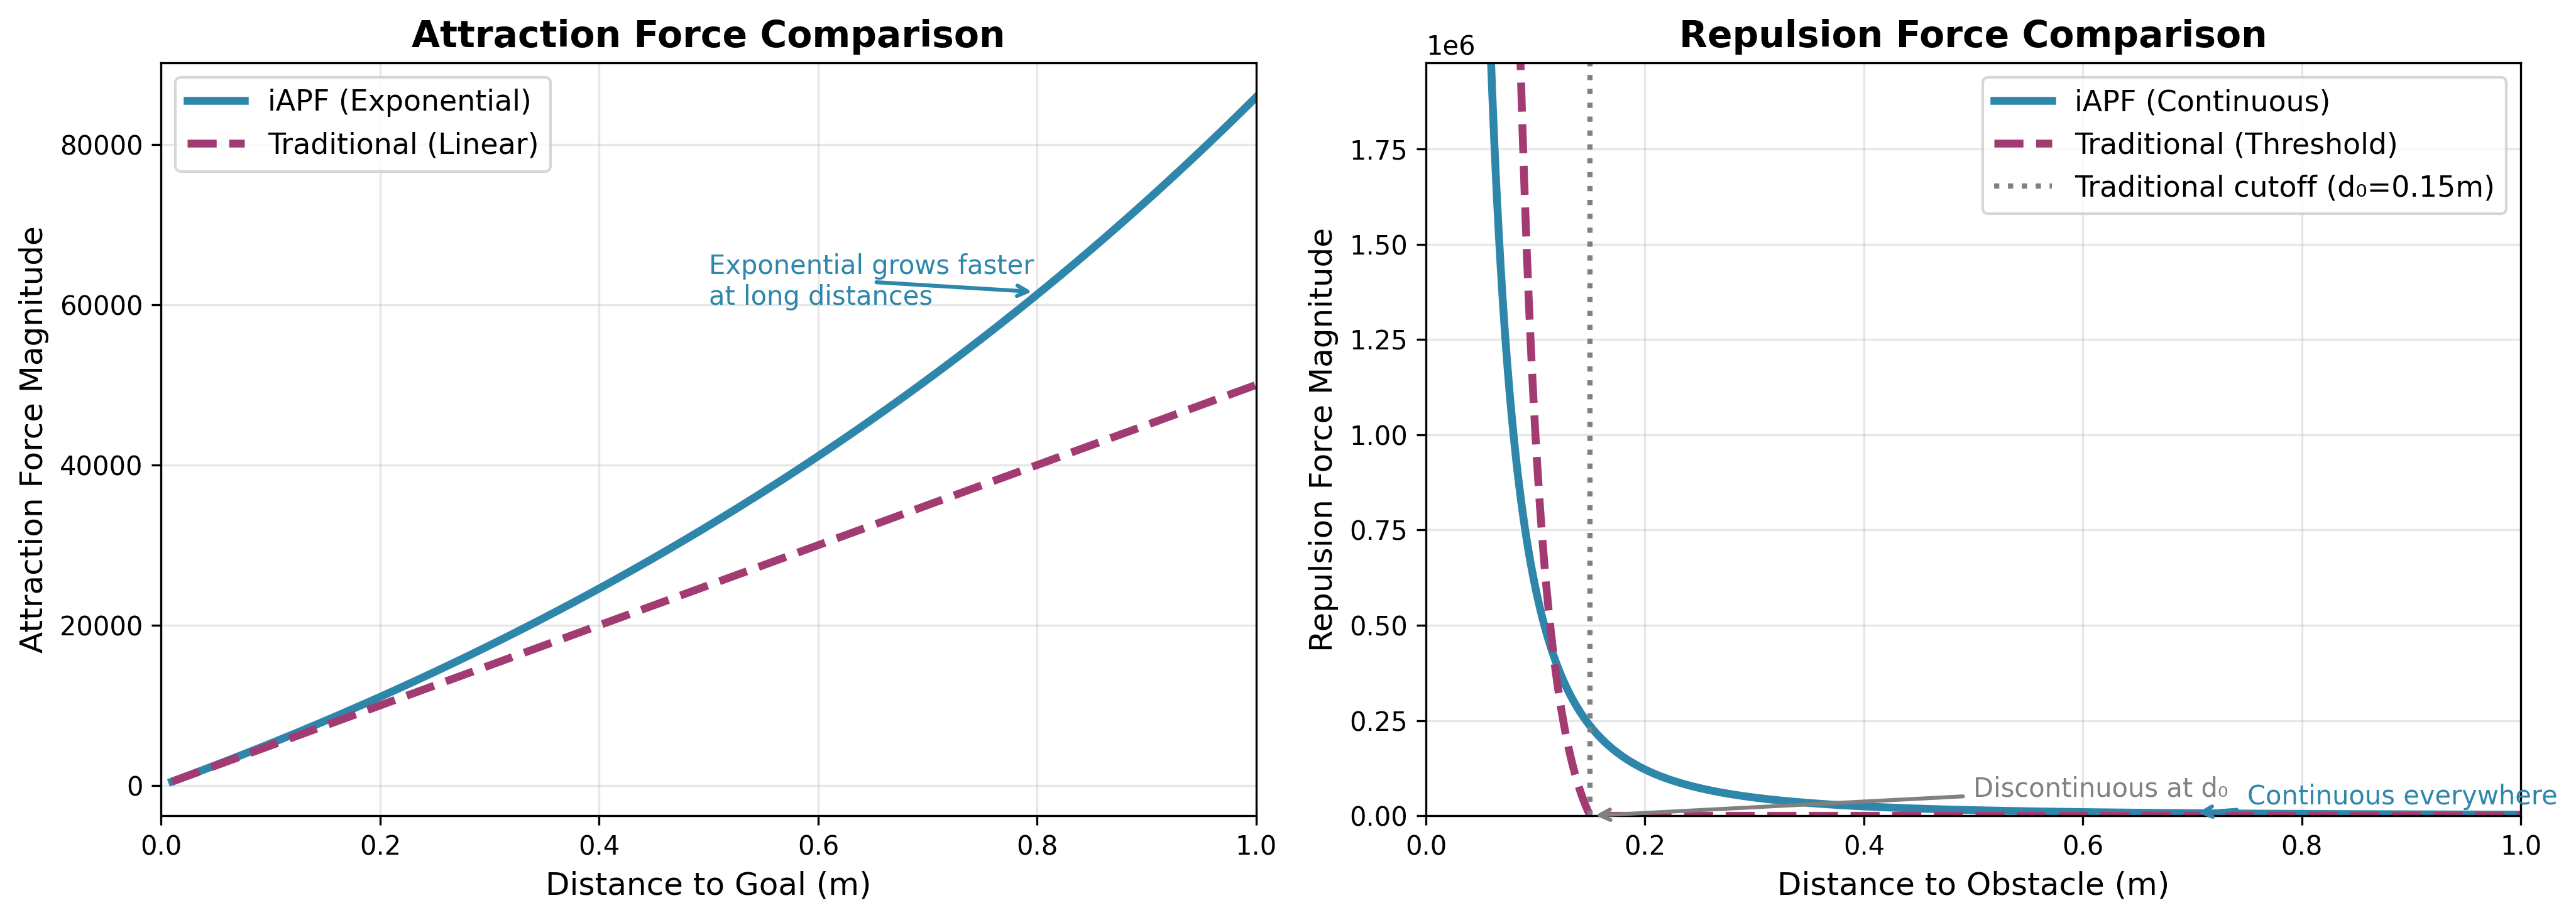
\includegraphics[width=0.8\linewidth]{Images/iapfAllocation/force_profile_comparison.png}
\caption{Force profile comparison: exponential attraction with adaptive gradient (left) against
linear attraction, and continuous repulsion eliminating the traditional threshold discontinuity
(right)~\citep{sk2025competitive}.}
\label{fig:cta_forces}
\end{figure}

\begin{figure}[htbp]
\centering
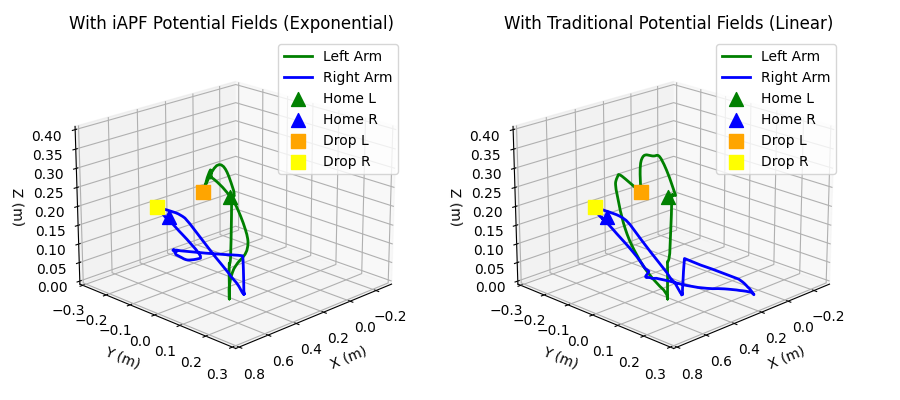
\includegraphics[width=0.75\linewidth]{Images/iapfAllocation/trajectory_comparison.png}
\caption{Dual-arm trajectories under a near-goal conflict with the tuned weights of this section:
iAPF (left) against the traditional APF~\citep{khatib1986real} (right)~\citep{sk2025competitive}.}
\label{fig:cta_trajcomp}
\end{figure}

Figure~\ref{fig:cta_forces} and Figure~\ref{fig:cta_trajcomp} reproduce, under competitive
allocation and the refined scaling of this section, the same qualitative comparison
Chapter~\ref{chap:iapf} established for the fixed-assignment case: the traditional APF's trajectory
deviates sharply when the repulsive force spikes at close range, while iAPF remains smooth,
confirming that neither the switch to competitive allocation nor the two-stage scaling refinement
disturbs the stable behaviour validated in Section~\ref{sec:iapf_validation}.

%% ============================================================
\section{Experimental Validation and Results}\label{sec:cta_results}
%% ============================================================

Validation proceeded in two stages: a simulation benchmark isolating the task-allocation mechanism
against three baselines, and hardware trials of the complete pipeline on homogeneous and
heterogeneous object sets.

%% ------------------------------------------------------------
\subsection{Simulation Benchmark of Allocation Strategies}\label{subsec:cta_simbench}
%% ------------------------------------------------------------

A simulation environment closely resembling the hardware workspace (Figure~\ref{fig:cta_simworkspace})
compared the proposed competitive allocation against market-based, round-robin, and the original
fixed nut-left/bolt-right allocation of Section~\ref{sec:iapf_priority}, over 100 trials, using the
three metrics of Figure~\ref{fig:cta_simmetrics}: distance efficiency (the inverse mean
object-to-arm distance), collision risk (detected trajectory intersections during simultaneous
operation), and coverage (the percentage of objects successfully allocated).

\begin{figure}[htbp]
\centering
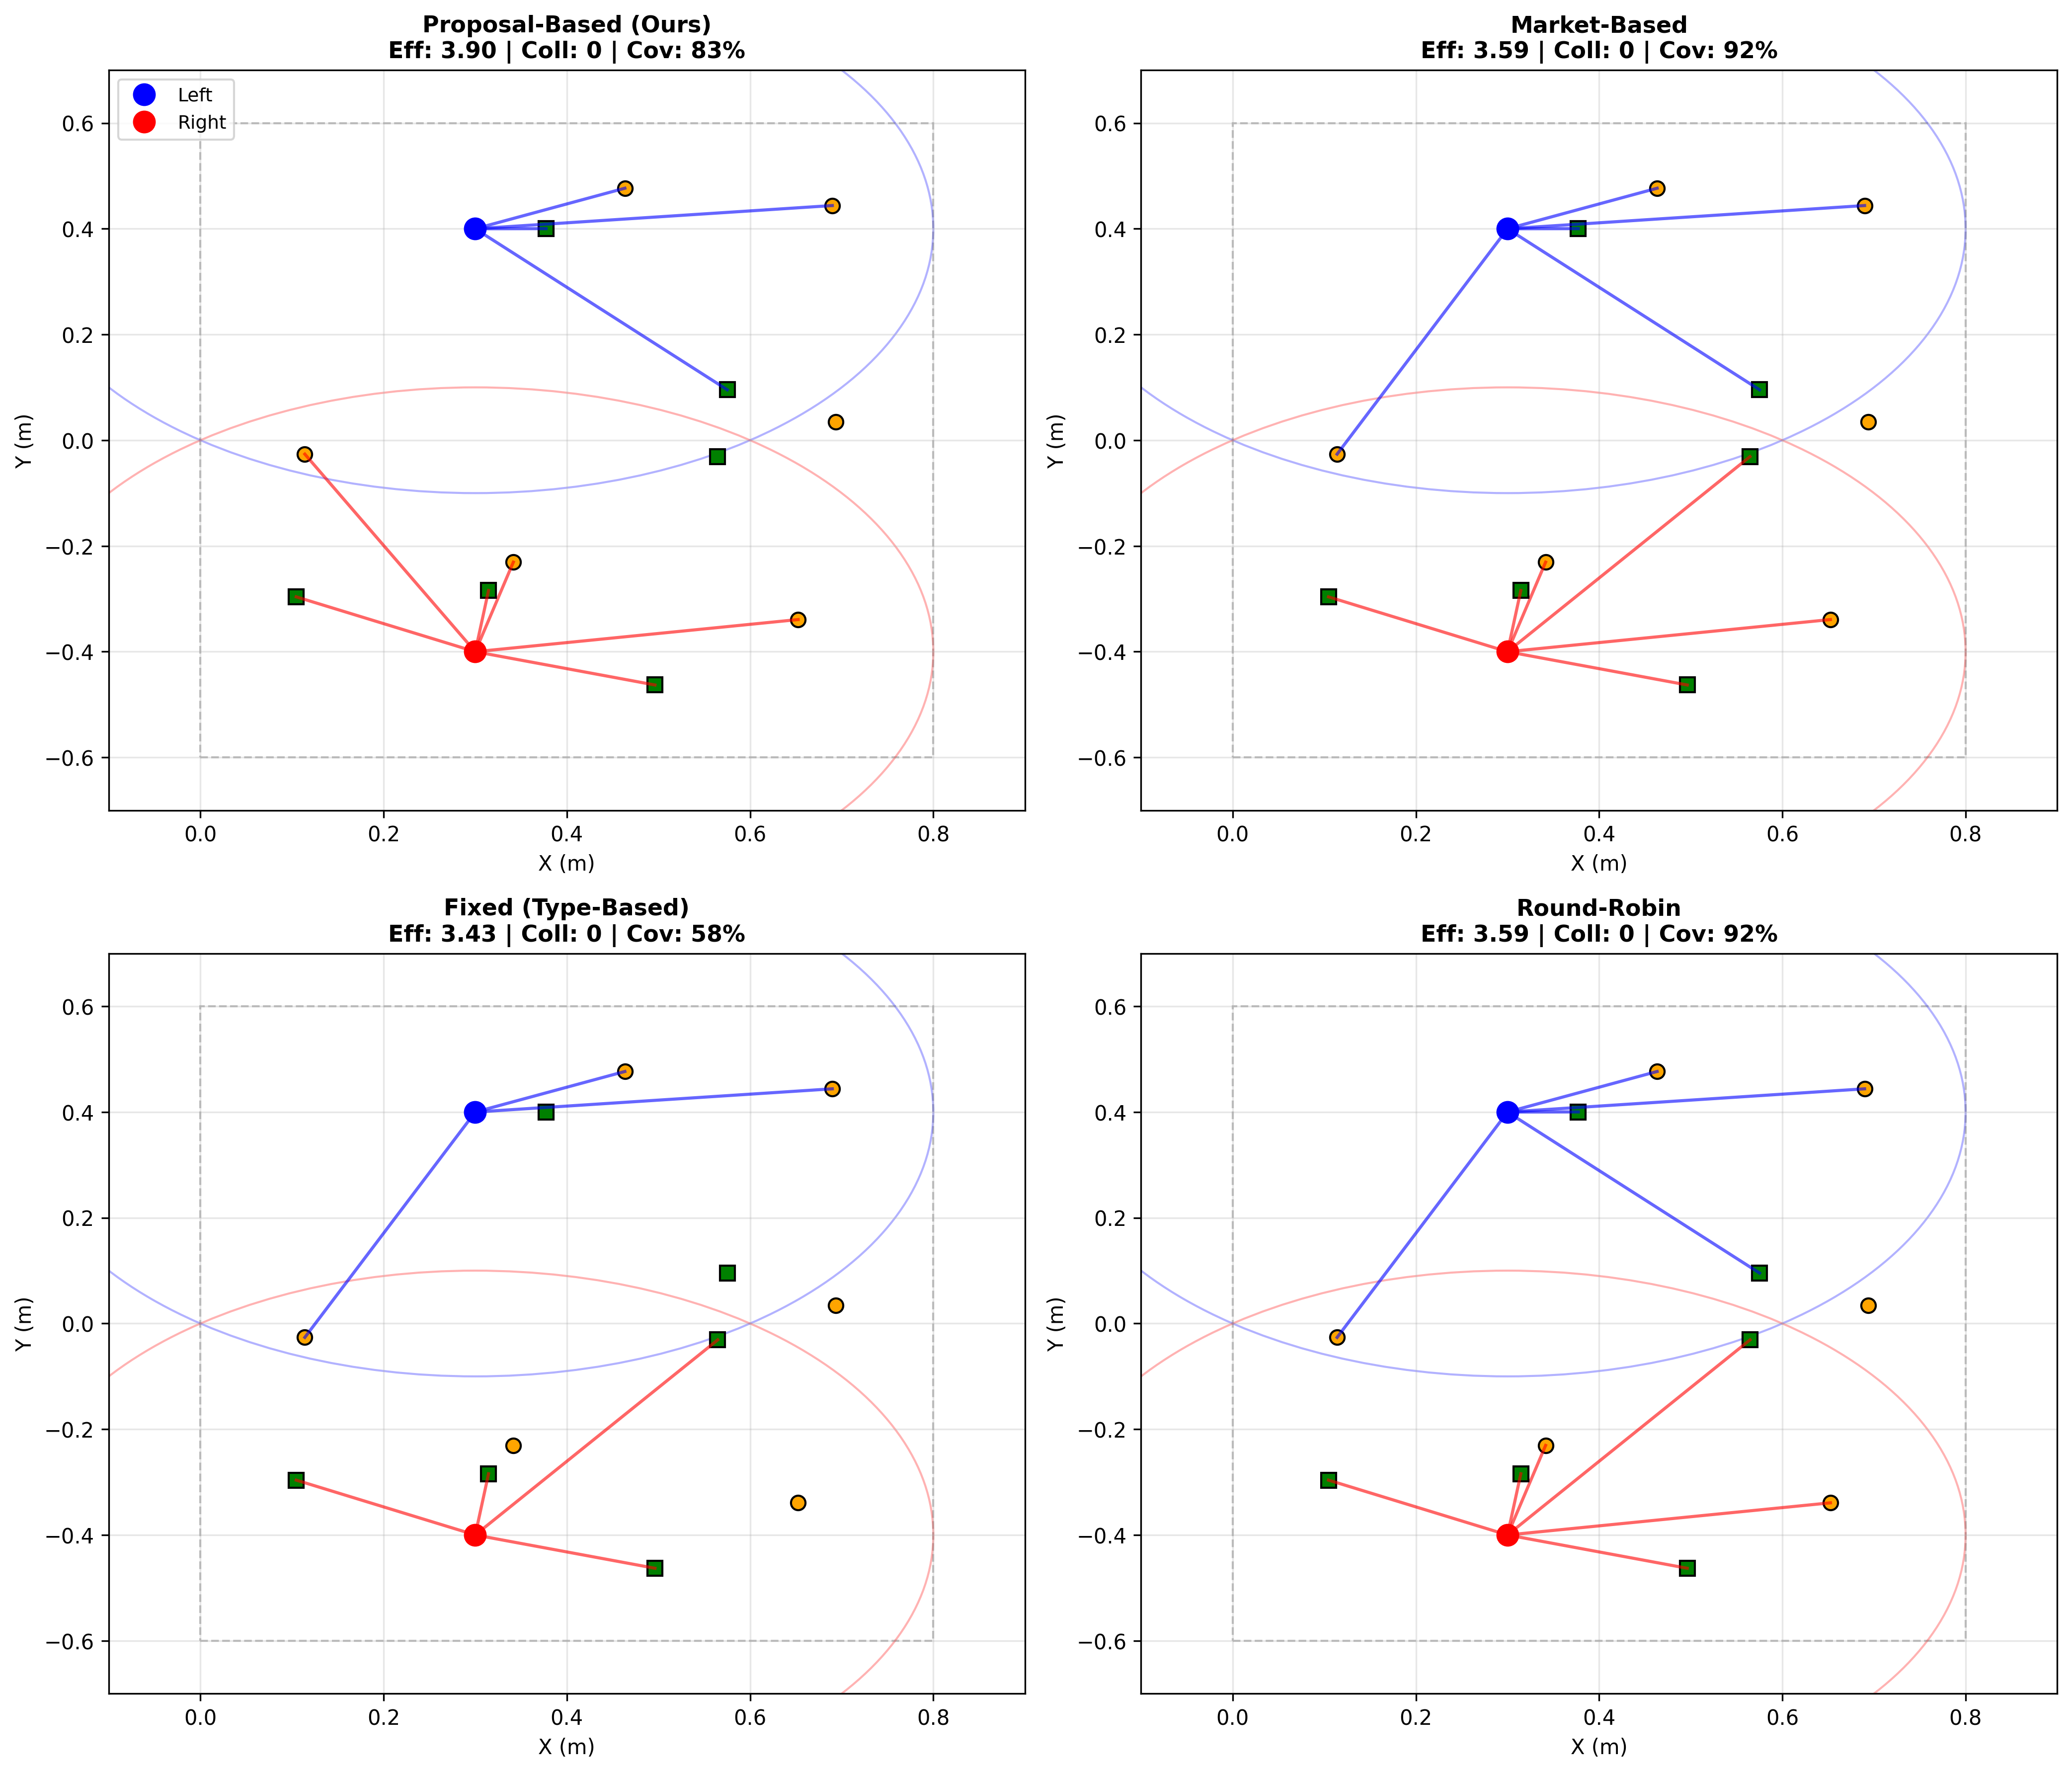
\includegraphics[width=0.7\linewidth]{Images/iapfAllocation/allocation_workspace_comparison.png}
\caption{Simulated dual-arm workspace comparing the four allocation strategies~\citep{sk2025competitive}.}
\label{fig:cta_simworkspace}
\end{figure}

\begin{figure}[htbp]
\centering
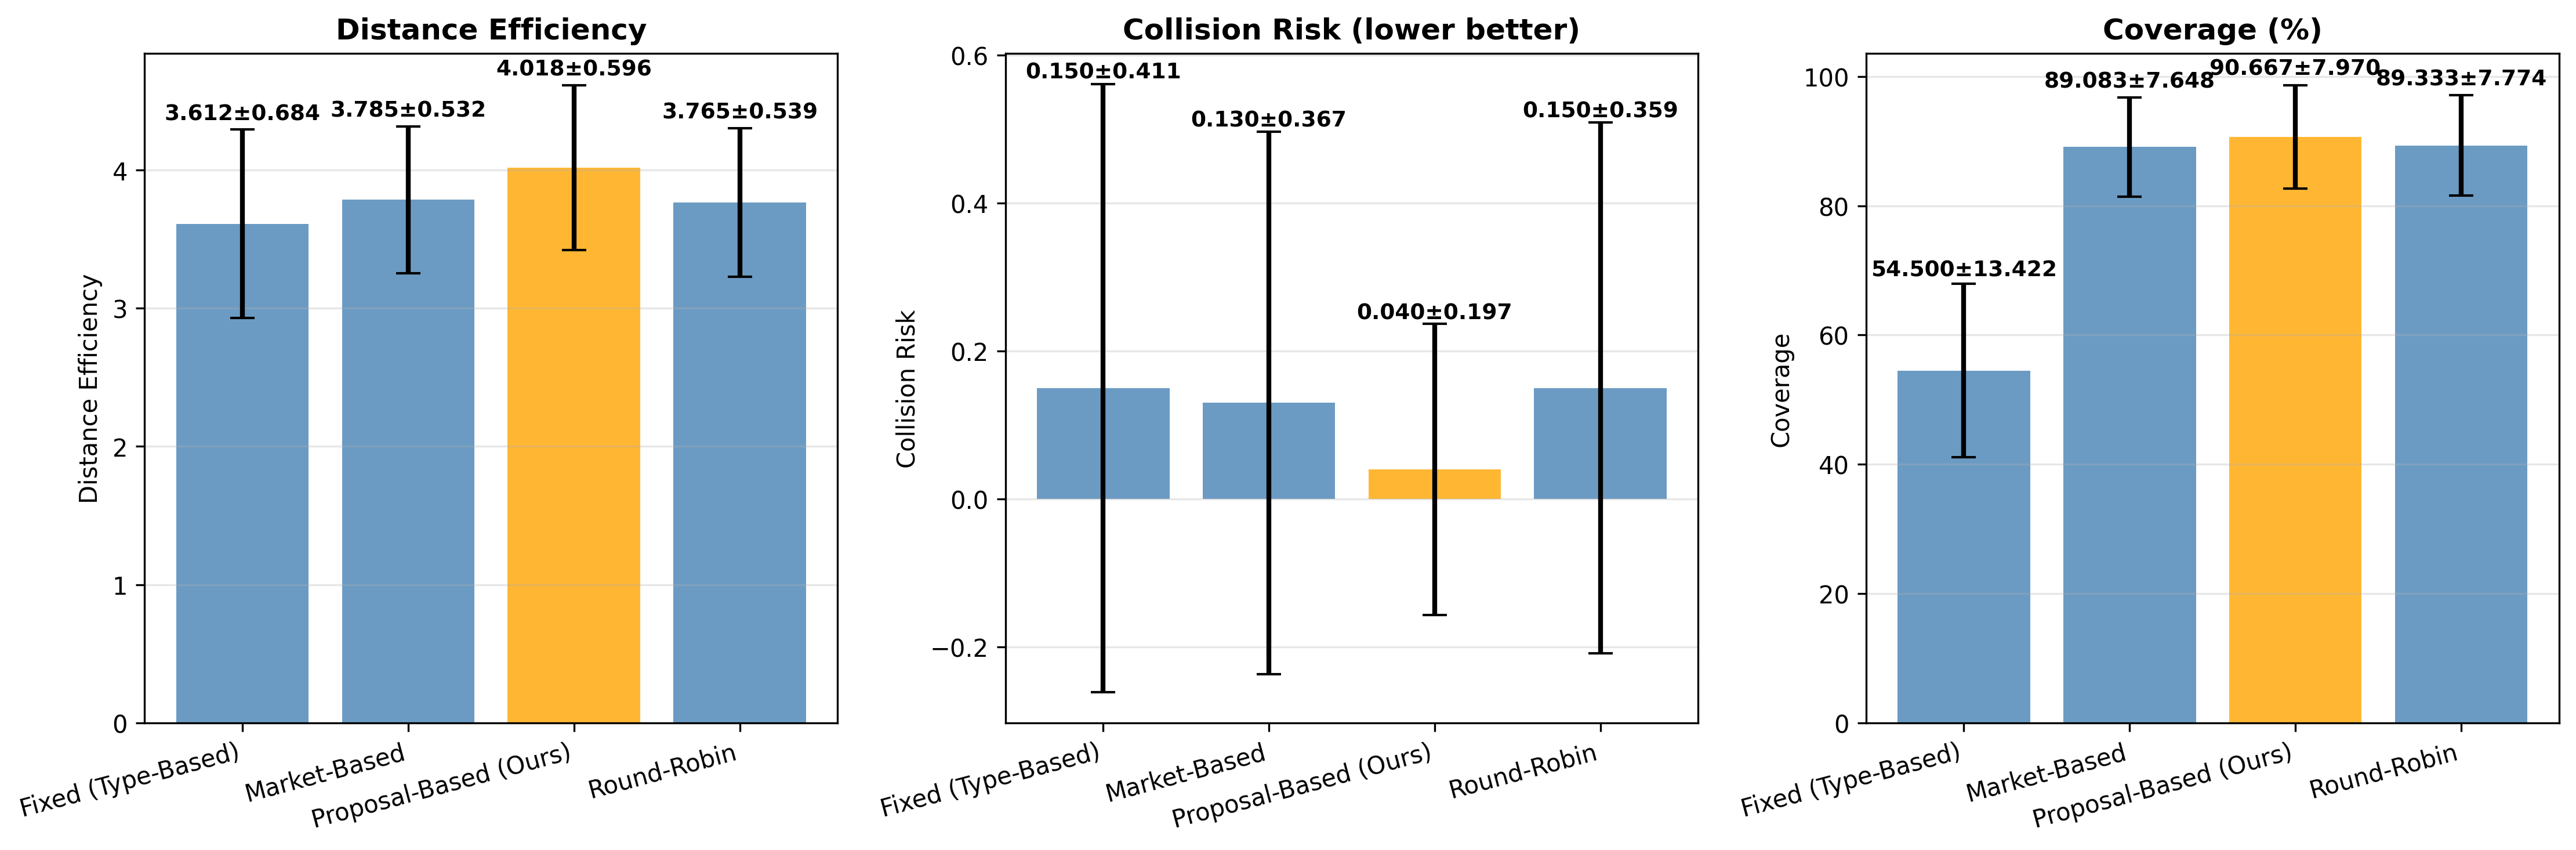
\includegraphics[width=\linewidth]{Images/iapfAllocation/allocation_metrics.png}
\caption{Distance efficiency, collision risk, and coverage across the four allocation
strategies~\citep{sk2025competitive}.}
\label{fig:cta_simmetrics}
\end{figure}

The proposed method reached a distance efficiency of $4.020 \pm 0.595$, ahead of market-based
($3.789 \pm 0.530$, a $6.1\%$ improvement), round-robin ($3.769 \pm 0.537$, $6.7\%$), and the
original fixed allocation ($3.618 \pm 0.681$, $11.1\%$), an improvement attributable to the
competitive updates of Equation~\eqref{eq:cta_update} replacing a previously proposed target
whenever a meaningfully closer object appears within the evaluation window, something neither
market-based bidding, which locks in immediately after each auction, nor round-robin, which ignores
proximity entirely, can do. Collision risk fell by $69\%$ against market-based
($0.040 \pm 0.197$ versus $0.130 \pm 0.367$) and $73\%$ against round-robin ($0.150 \pm 0.359$),
since both baselines assign objects without checking whether simultaneous assignments create
intersecting trajectories, a check the spatial conflict resolution of
Equation~\eqref{eq:cta_conflict} performs directly. Coverage remained above $89\%$ for every
competitive method, while the fixed nut-left/bolt-right allocation reached only
$54.9 \pm 13.7\%$, since its rigid per-arm type constraint, exactly gap G5, leaves objects outside
an arm's designated type unassigned regardless of reachability.

%% ------------------------------------------------------------
\subsection{Hardware: Homogeneous Object Scenarios}\label{subsec:cta_hwhomog}
%% ------------------------------------------------------------

\begin{figure}[htbp]
\centering
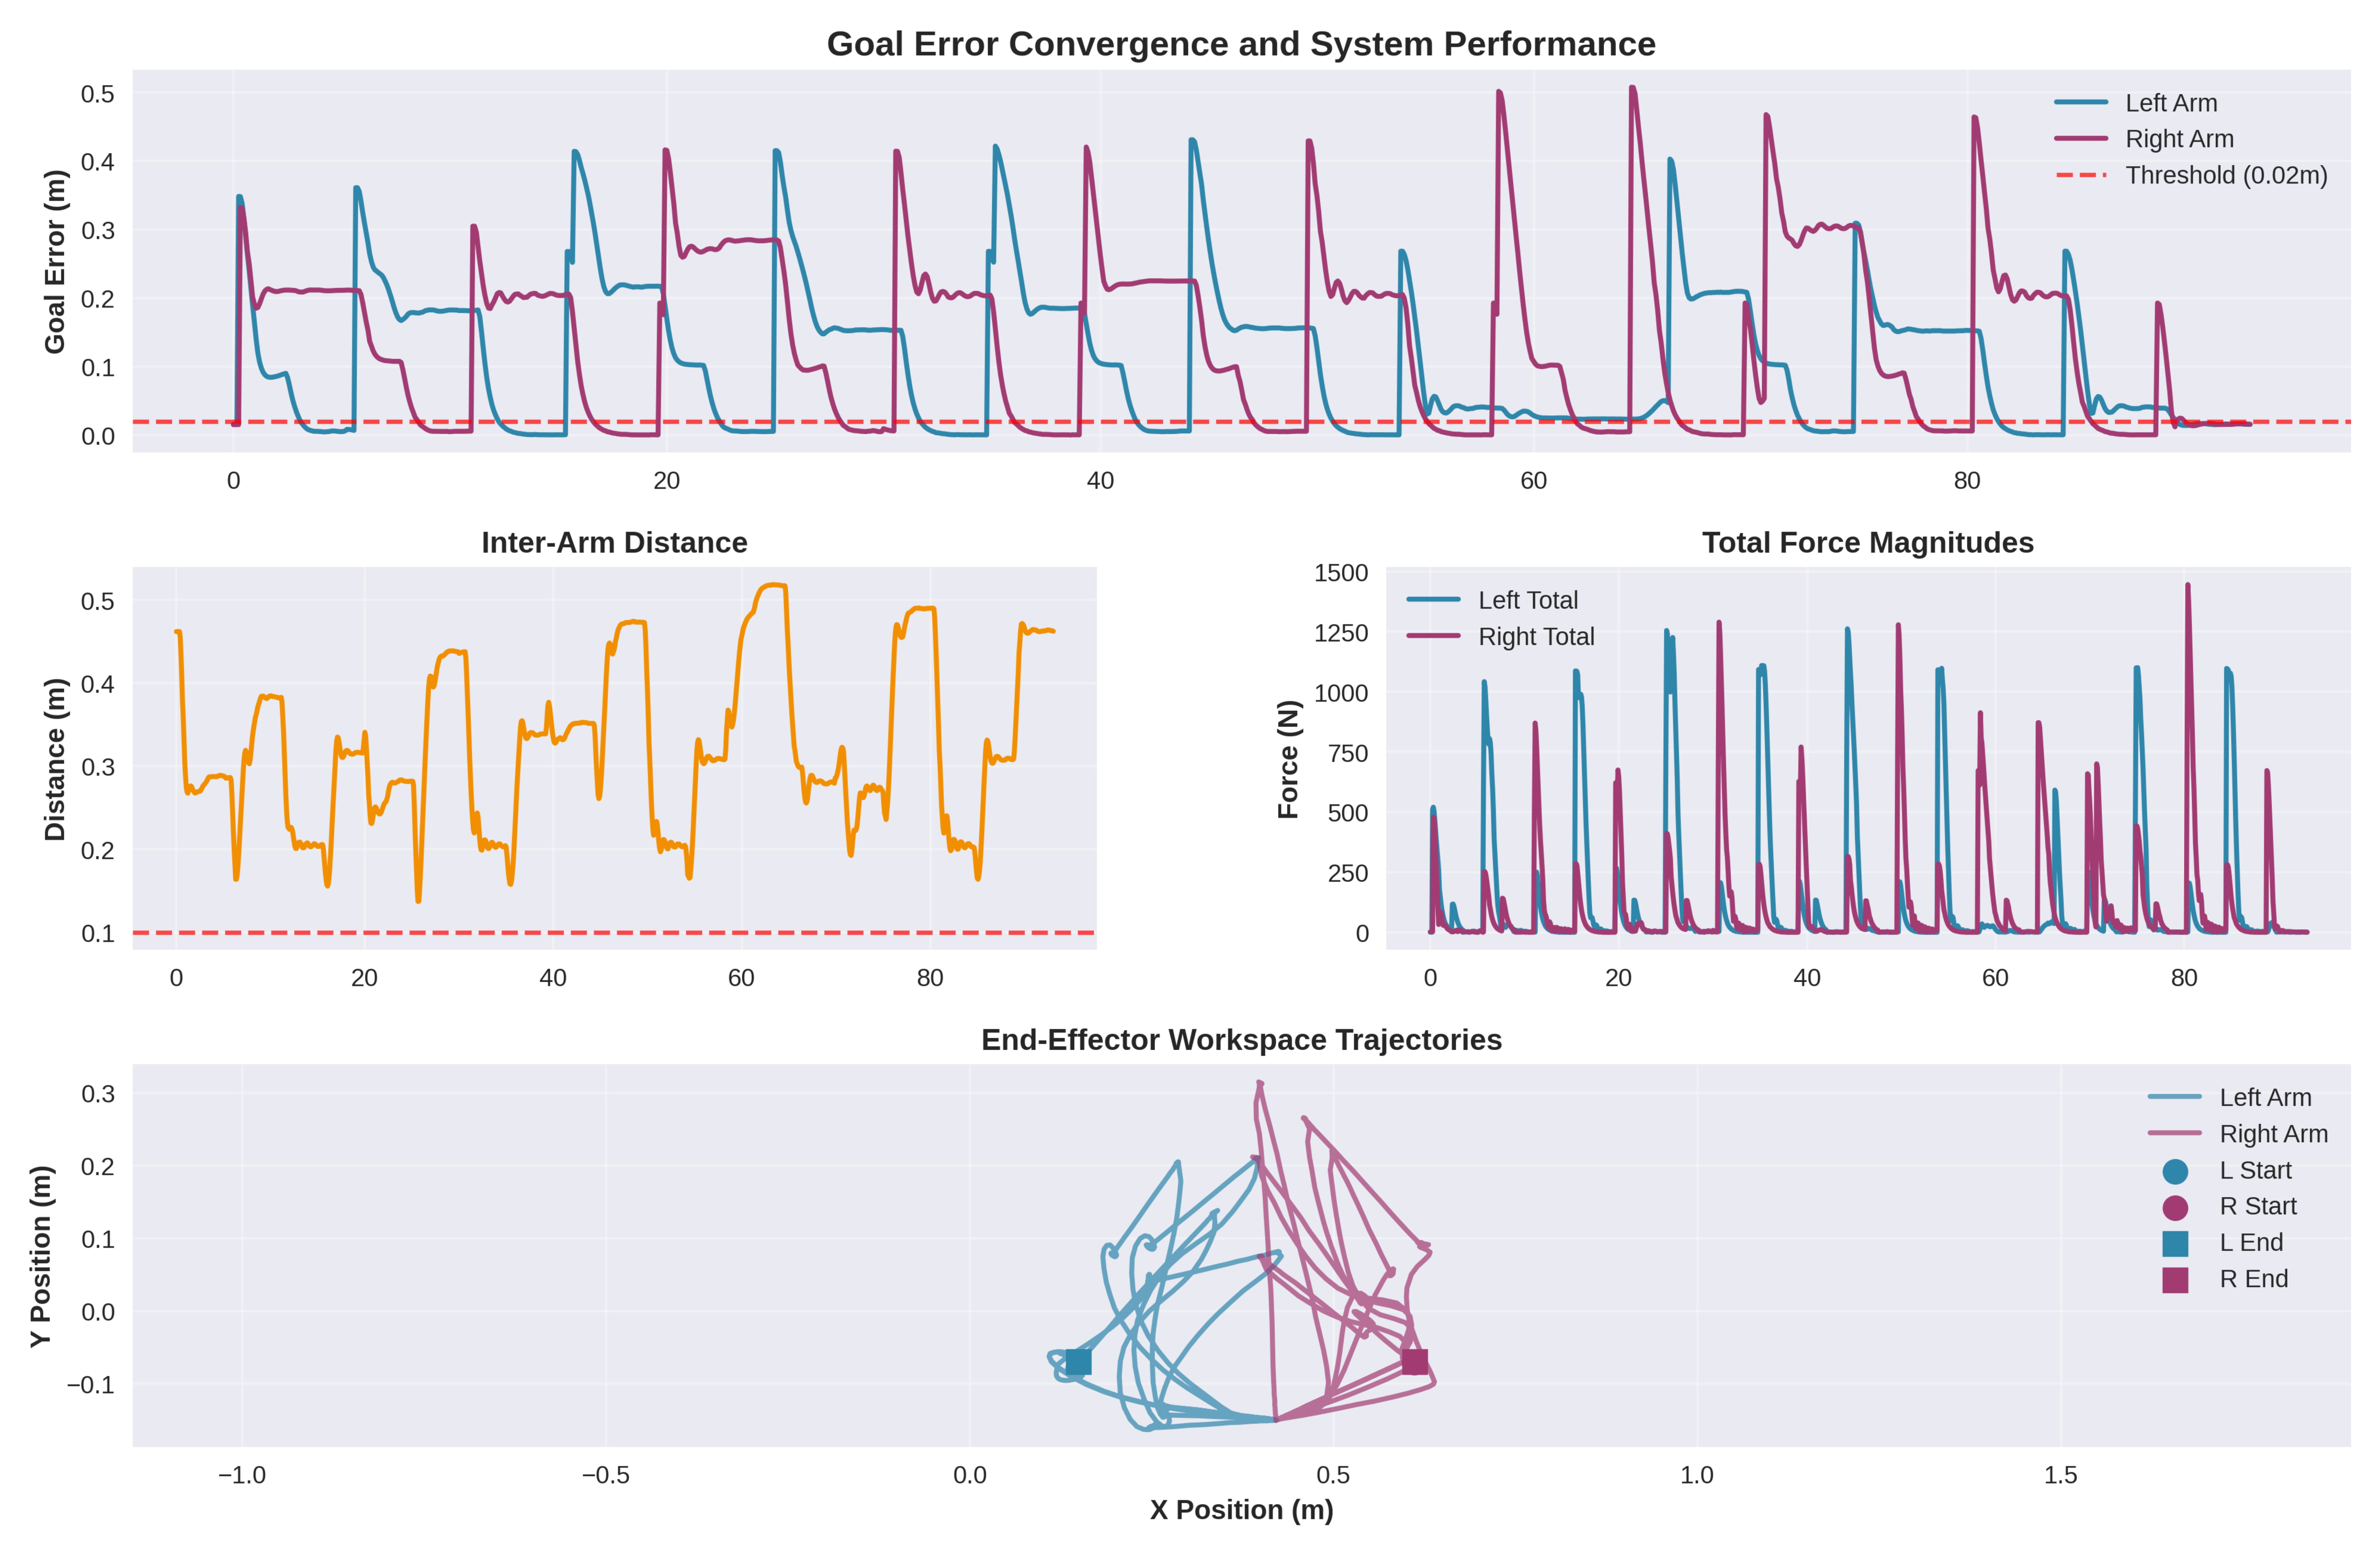
\includegraphics[width=0.75\linewidth]{Images/iapfAllocation/dynamic_single_object_analysis.jpg}
\caption{Dual-arm system analysis for competitive task allocation, single object type
(homogeneous)~\citep{sk2025competitive}.}
\label{fig:cta_dynhomog}
\end{figure}

\begin{figure}[htbp]
\centering
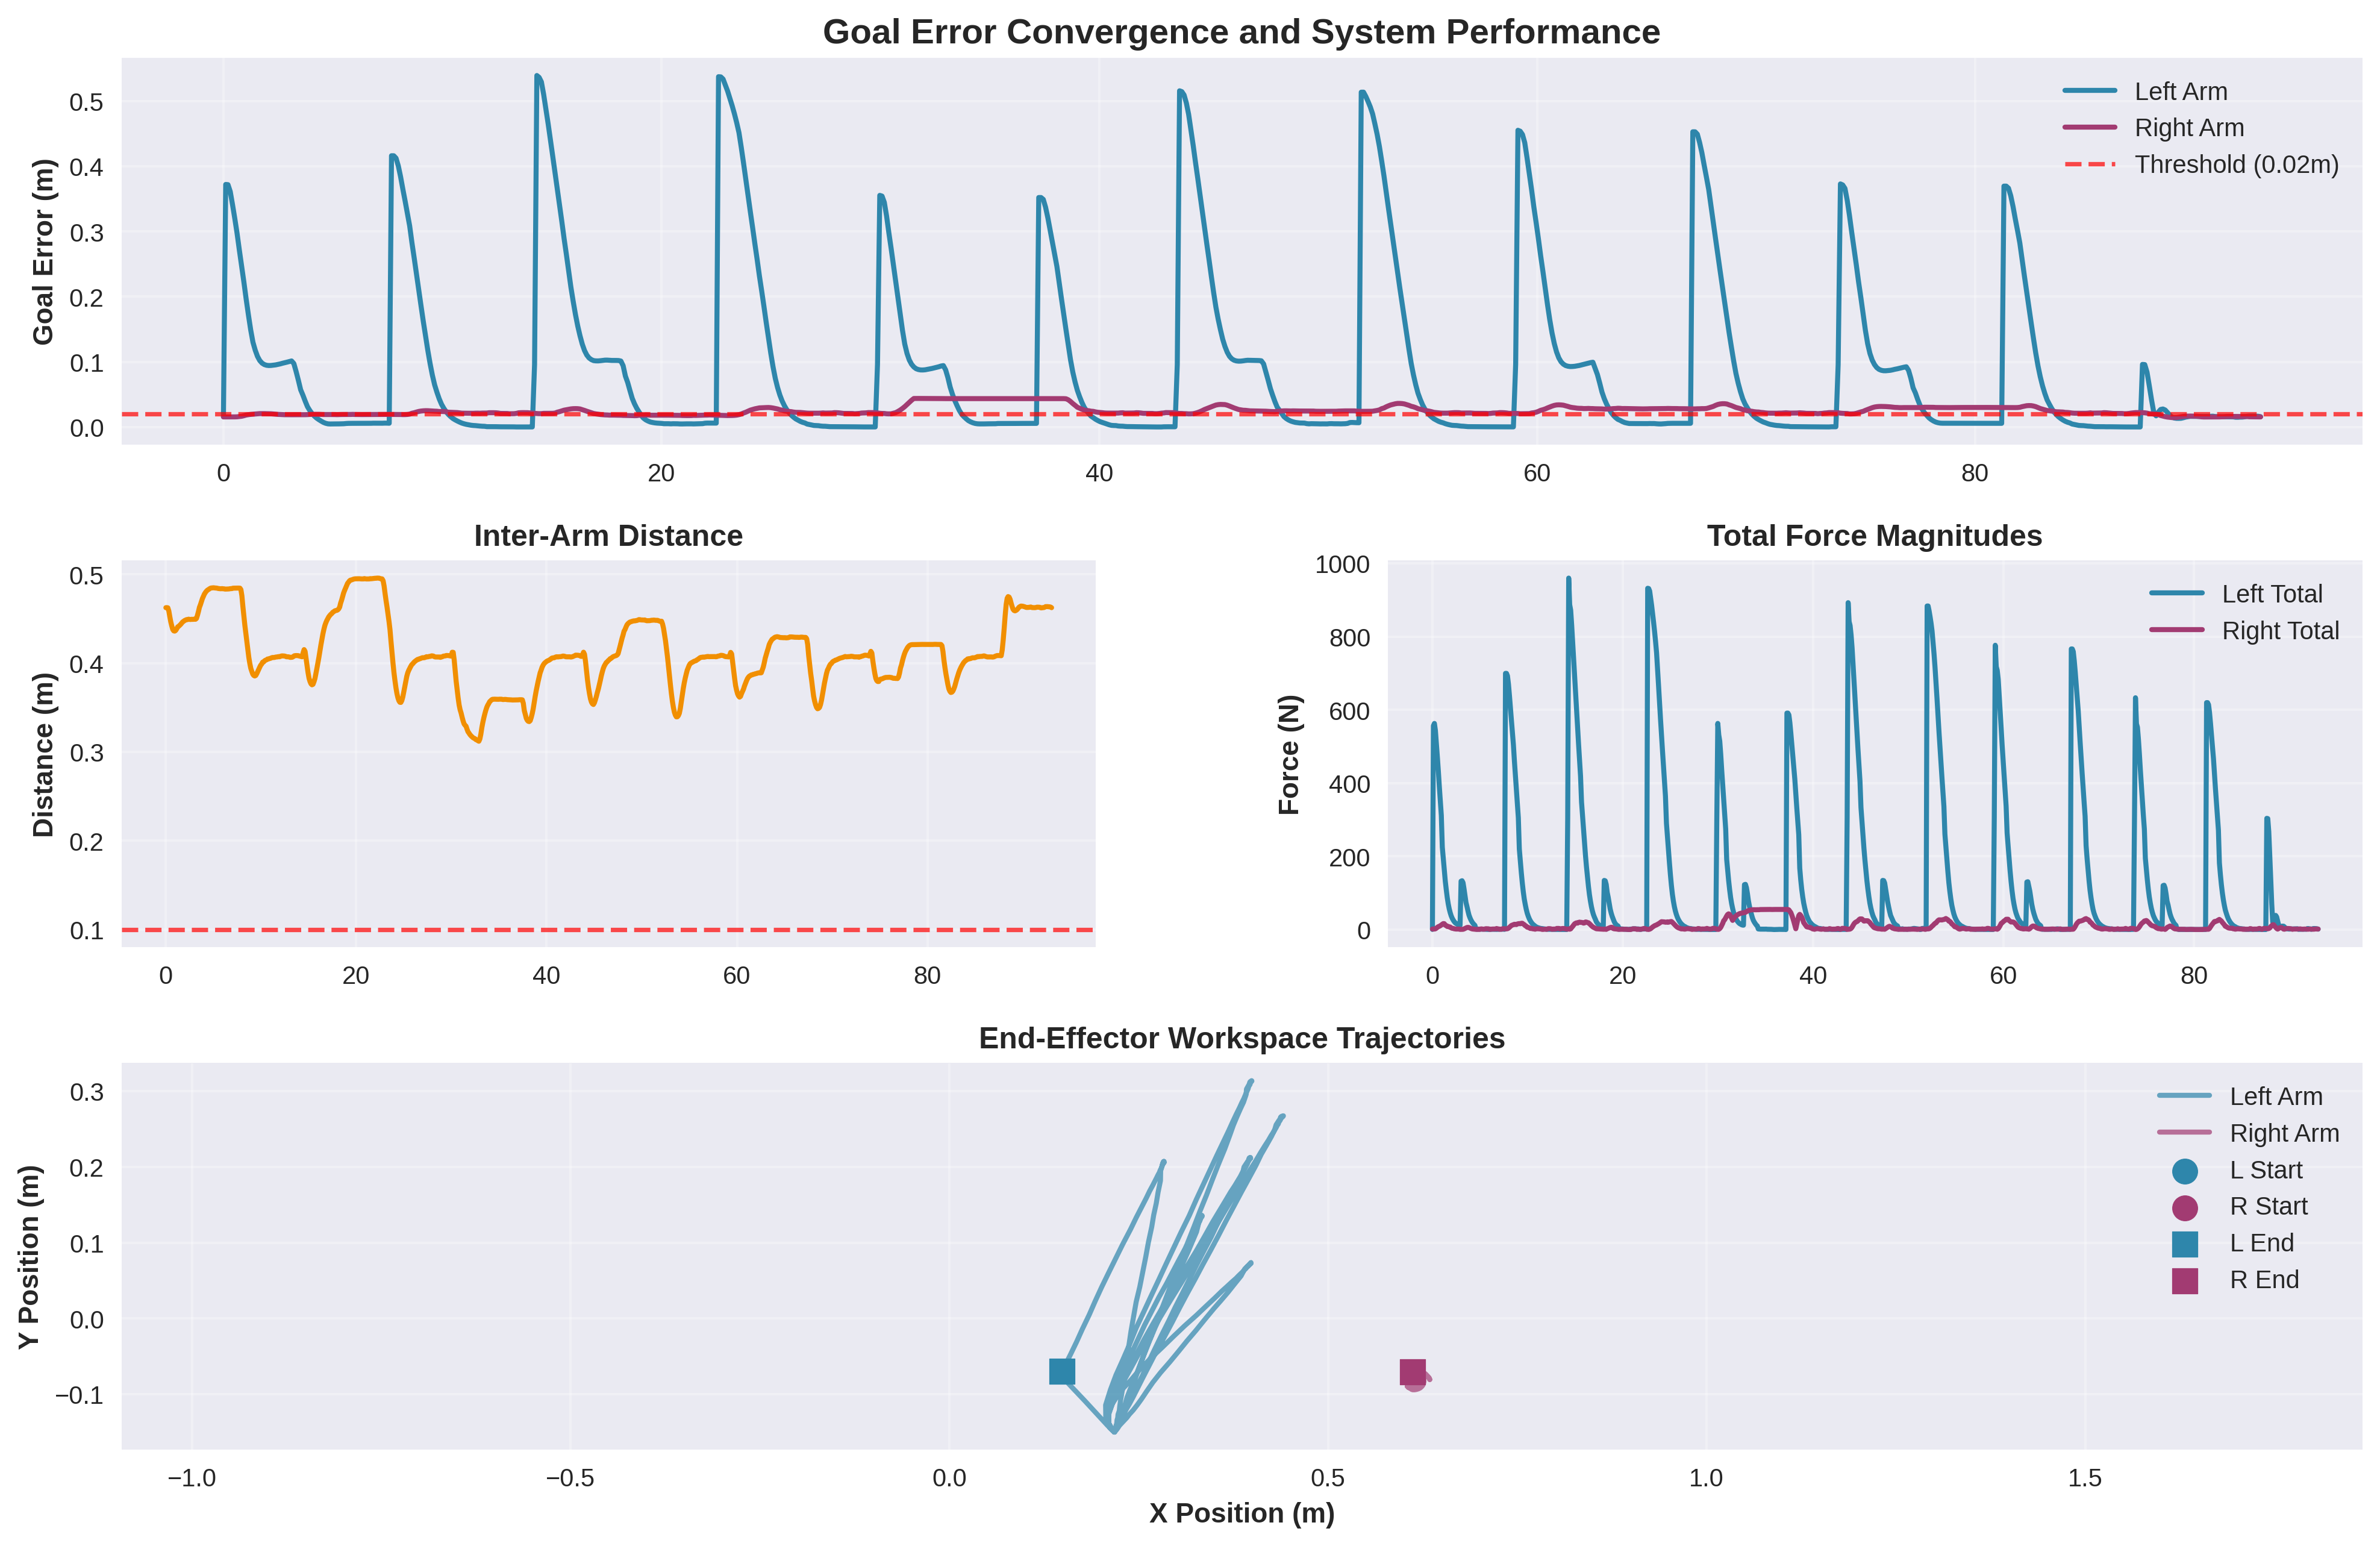
\includegraphics[width=0.75\linewidth]{Images/iapfAllocation/fixed_single_object_analysis.png}
\caption{Dual-arm system analysis for the original fixed task allocation, single object type
(homogeneous)~\citep{sk2025competitive}.}
\label{fig:cta_fixedhomog}
\end{figure}

Table~\ref{tab:cta_homogeneous} compares the complete hardware pipeline against the original fixed
allocation over ten trials with a single object type. Competitive allocation reaches an average
velocity of $\approx 0.116$\,m/s against $\approx 0.078$\,m/s for fixed allocation, a
$\approx 47\%$ improvement, because both arms contribute to every trial rather than one arm
handling all objects of its assigned type while the other sits idle, visible directly in the
contrast between Figure~\ref{fig:cta_dynhomog} and Figure~\ref{fig:cta_fixedhomog}.

\begin{table}[htbp]
\centering
\caption{Hardware comparison, homogeneous object scenarios (mean $\pm$ SD, $n=10$ trials).}
\label{tab:cta_homogeneous}
\begin{tabular}{llccc}
\toprule
\textbf{Method} & \textbf{Scenario} & \textbf{Distance (m)} & \textbf{Time (s)} & \textbf{Velocity (m/s)} \\
\midrule
\multirow{2}{*}{Competitive~\citep{sk2025competitive}} & Bolt-only & $7.60 \pm 0.082$ & $65.13 \pm 2.01$ & $0.116 \pm 0.003$ \\
                         & Nut-only  & $7.88 \pm 0.143$ & $67.87 \pm 1.06$ & $0.116 \pm 0.0002$ \\
\midrule
\multirow{2}{*}{Fixed~\citep{surya2025iapf}}   & Bolt-only & $6.61 \pm 0.016$ & $84.65 \pm 0.13$ & $0.078 \pm 0.0001$ \\
                         & Nut-only  & $6.42 \pm 0.010$ & $82.15 \pm 0.08$ & $0.078 \pm 0.0001$ \\
\bottomrule
\end{tabular}
\end{table}

%% ------------------------------------------------------------
\subsection{Hardware: Heterogeneous Object Scenarios}\label{subsec:cta_hwheterog}
%% ------------------------------------------------------------

\begin{figure}[htbp]
\centering
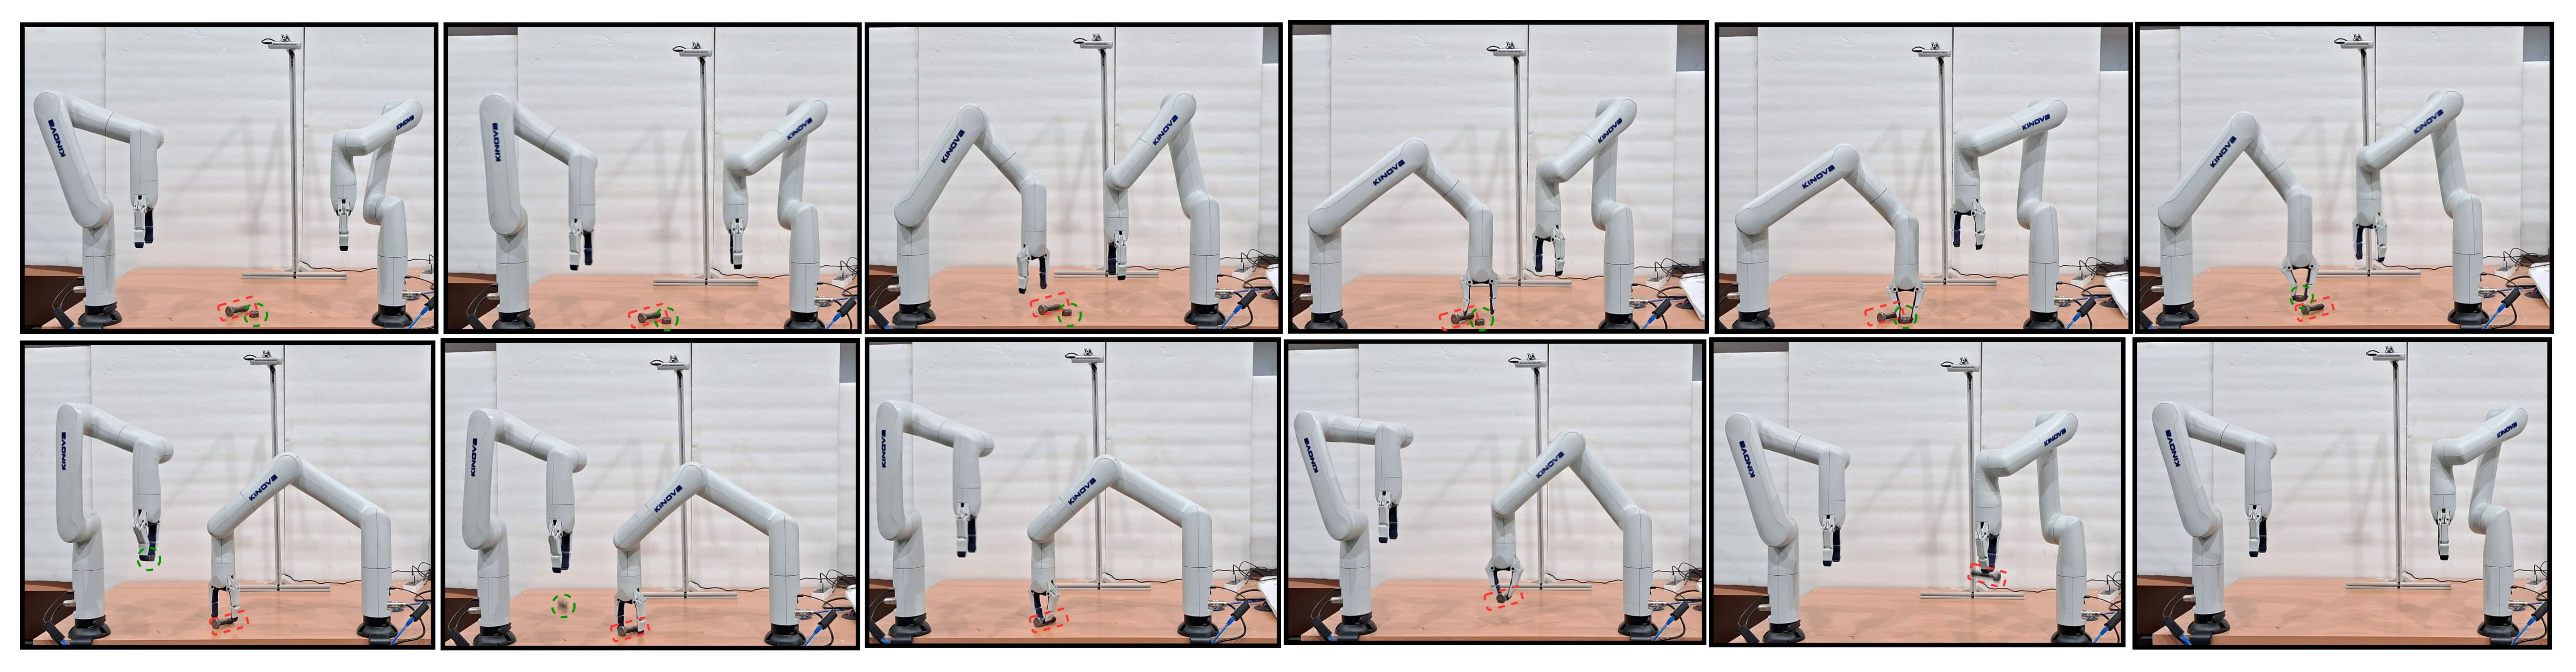
\includegraphics[width=0.7\linewidth]{Images/iapfAllocation/near_goal_conflict_sequence.jpg}
\caption{Dual-arm sequential movements under competitive allocation, with iAPF resolving
conflicting near-goal components~\citep{sk2025competitive}.}
\label{fig:cta_seqconflict}
\end{figure}

\begin{figure}[htbp]
\centering
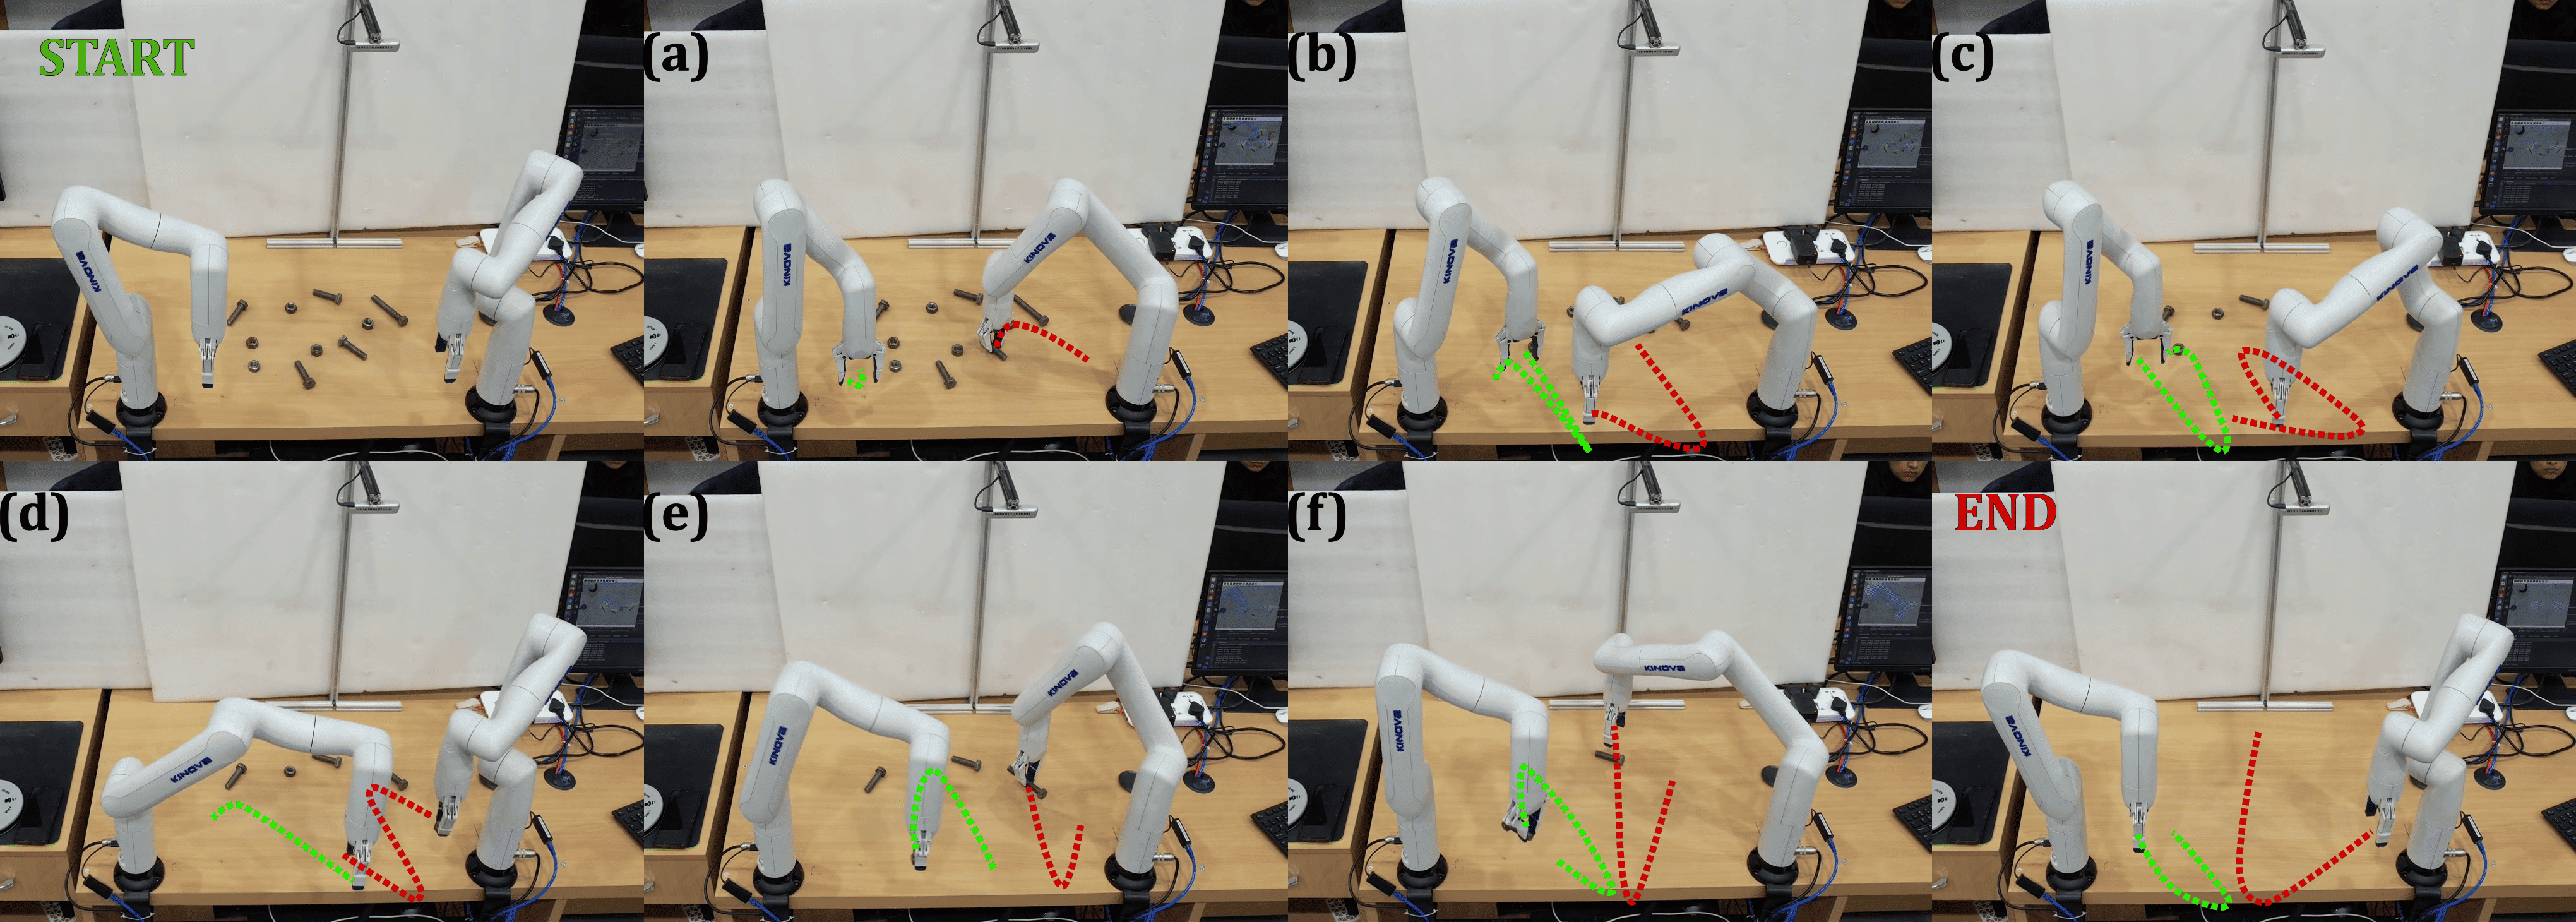
\includegraphics[width=0.75\linewidth]{Images/iapfAllocation/sorting_sequence.png}
\caption{Complete dual-arm sorting sequence from home through simultaneous pick-and-place and back
to home, with zero collision events~\citep{sk2025competitive}.}
\label{fig:cta_sortseq}
\end{figure}

Table~\ref{tab:cta_heterogeneous} reports mixed-object trials, twelve objects per trial (six nuts,
six bolts) in a compact arrangement, comparing all four strategies. The original fixed allocation
reports the highest average velocity, but this is an artefact of partial coverage
($\approx 55\%$): its type-constrained arms complete only the subset of objects within their own
reachable, high-density zone and leave the rest unassigned, rather than genuinely outperforming the
alternatives. Among the methods achieving full coverage ($>89\%$), the proposed method
($15.49$\,m, $135.42$\,s) improves on market-based allocation by $8.0\%$ in distance and $11.0\%$ in
time, and on round-robin by $15.9\%$ and $22.7\%$ respectively, consistent with the simulation
results of Section~\ref{subsec:cta_simbench}.

\begin{table}[htbp]
\centering
\caption{Hardware comparison, heterogeneous (mixed) object scenarios, 12 objects per trial
(mean $\pm$ SD, $n=10$ trials).}
\label{tab:cta_heterogeneous}
\begin{tabular}{lccc}
\toprule
\textbf{Method} & \textbf{Distance (m)} & \textbf{Time (s)} & \textbf{Velocity (m/s)} \\
\midrule
Competitive (proposed)~\citep{sk2025competitive} & $15.49 \pm 0.226$ & $135.42 \pm 0.485$ & $0.114 \pm 0.001$ \\
Market-based~\citep{quinton2023market}       & $16.85 \pm 0.315$ & $152.10 \pm 1.450$ & $0.110 \pm 0.002$ \\
Round-robin~\citep{korsah2013comprehensive}        & $18.42 \pm 0.412$ & $175.30 \pm 2.100$ & $0.105 \pm 0.003$ \\
Fixed (original~\citep{surya2025iapf}, partial coverage $\approx 55\%$) & $12.57 \pm 0.181$ & $98.40 \pm 0.800$ & $0.128 \pm 0.001$ \\
\bottomrule
\end{tabular}
\end{table}

\begin{figure}[htbp]
\centering
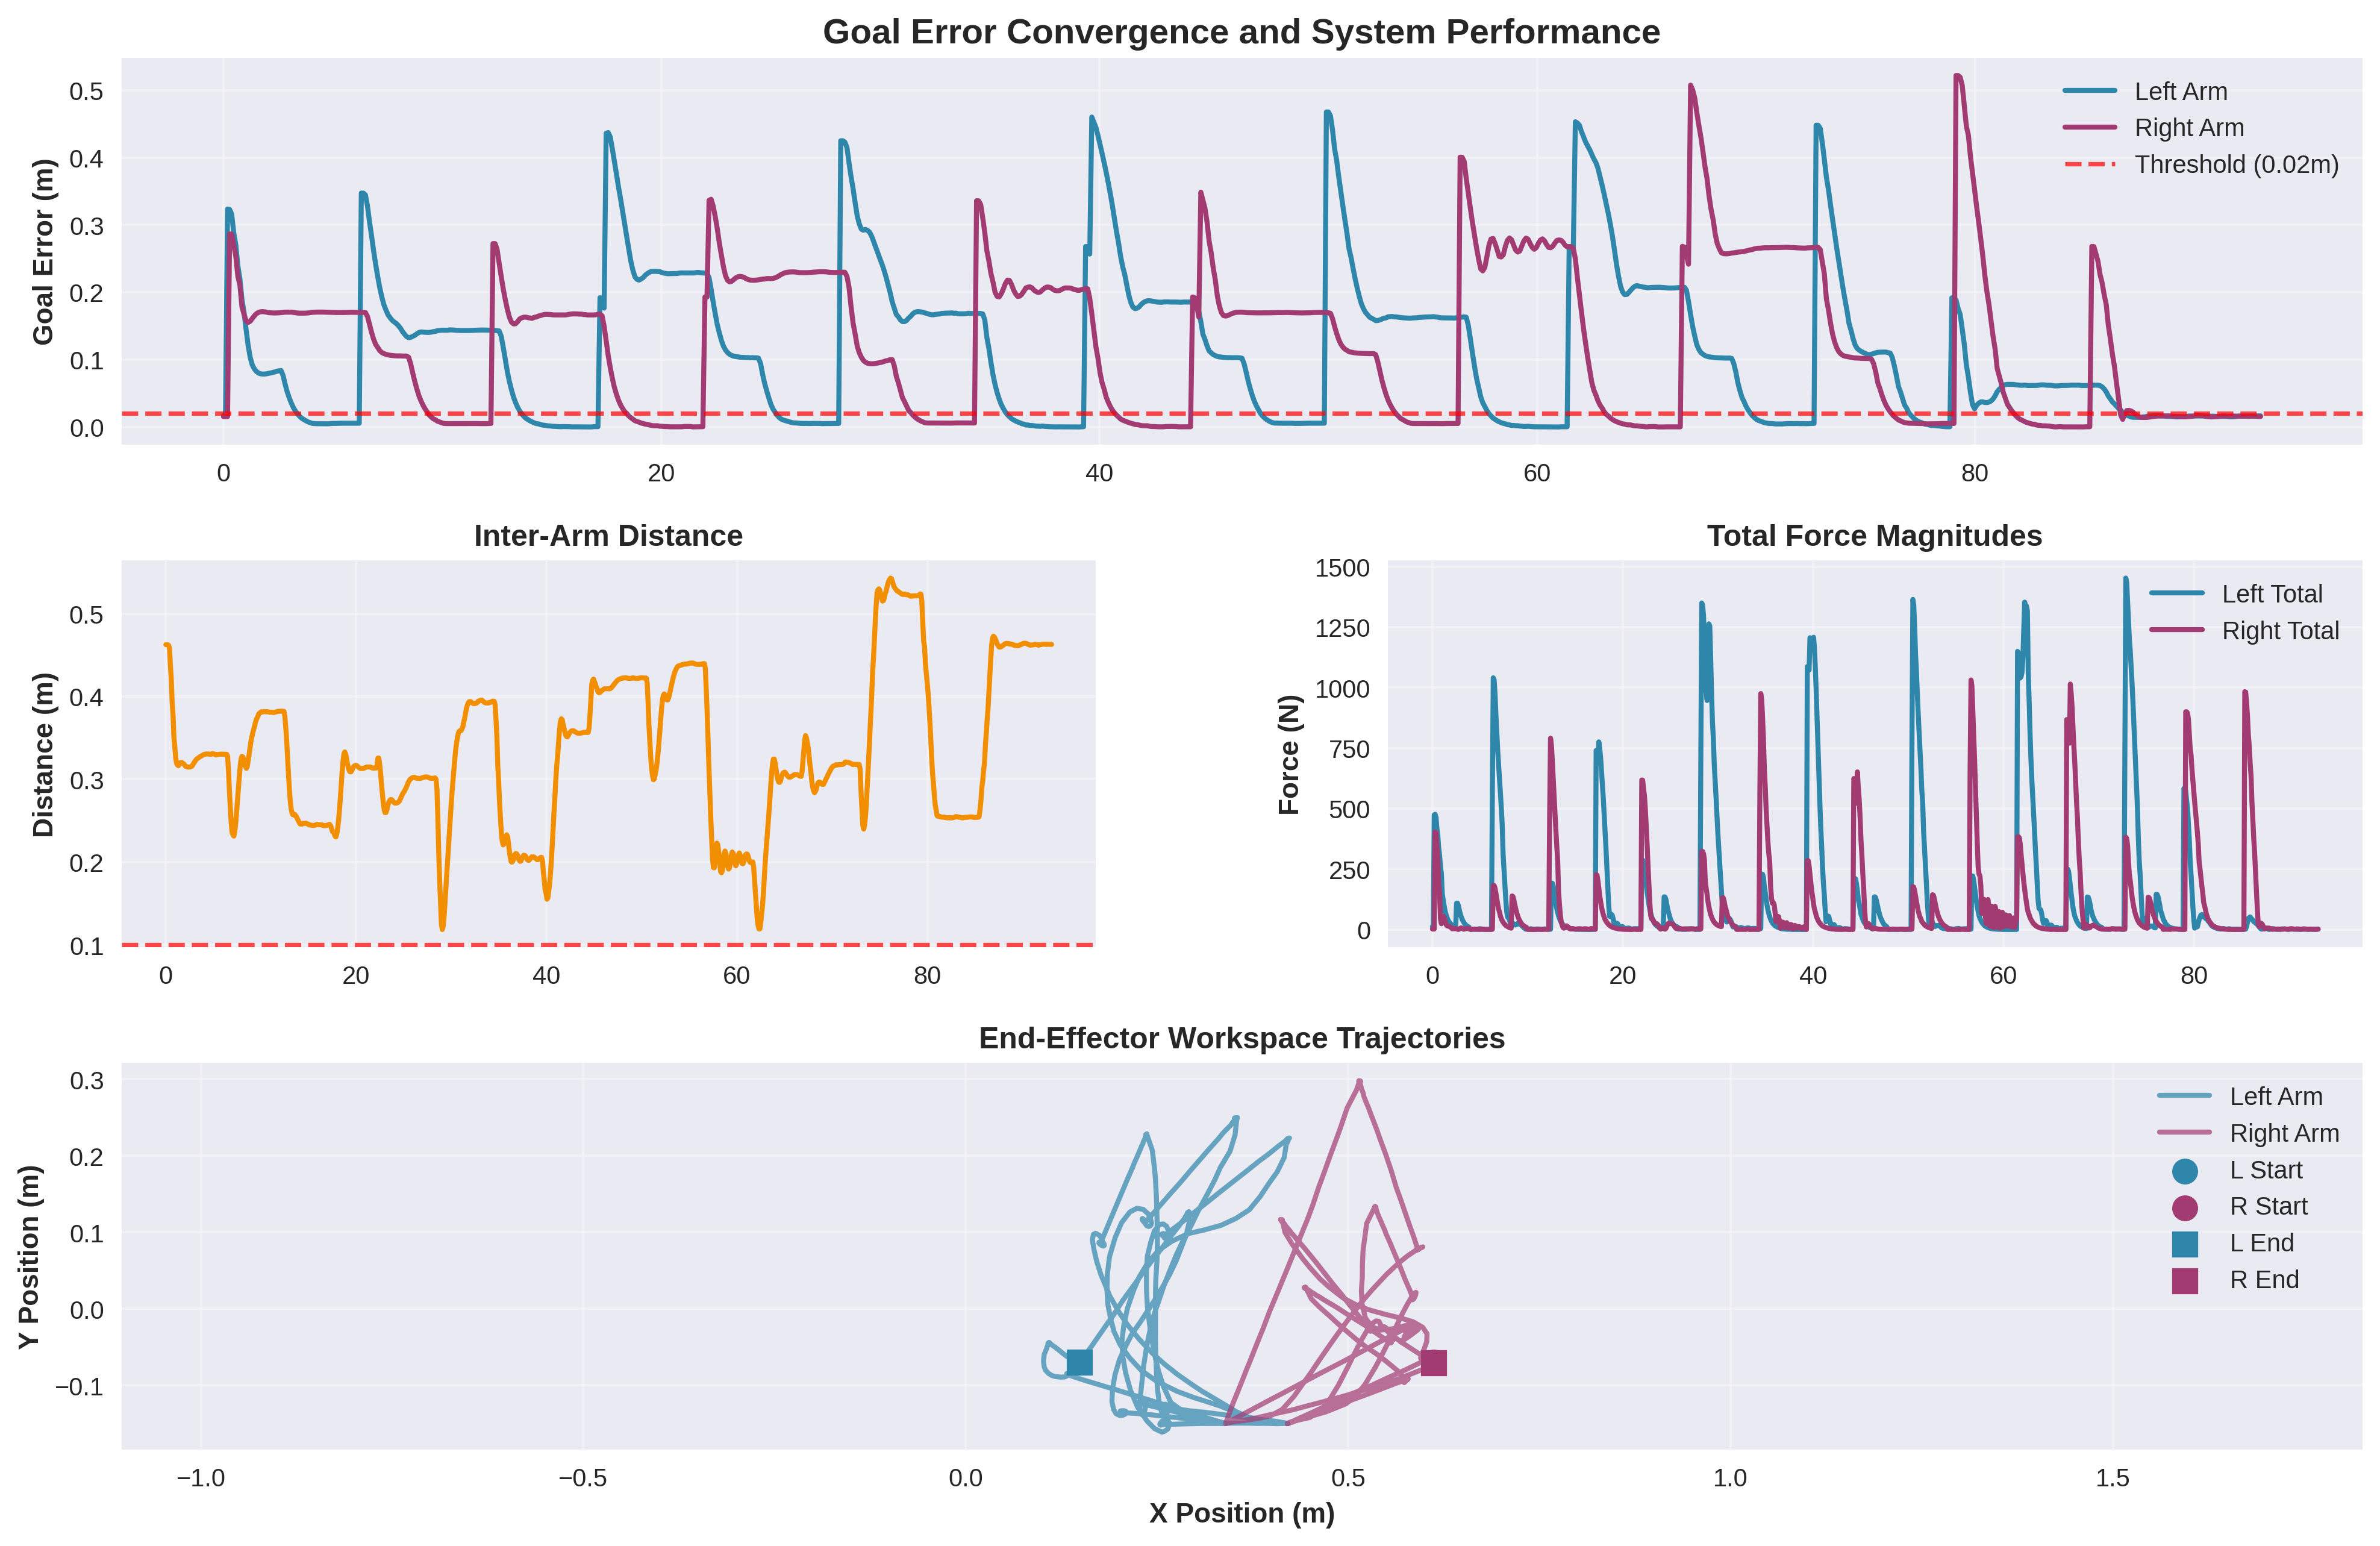
\includegraphics[width=0.75\linewidth]{Images/iapfAllocation/dynamic_mixed_analysis.png}
\caption{Combined dual-arm system analysis, competitive task allocation, mixed
objects~\citep{sk2025competitive}.}
\label{fig:cta_dynmixed}
\end{figure}

\begin{figure}[htbp]
\centering
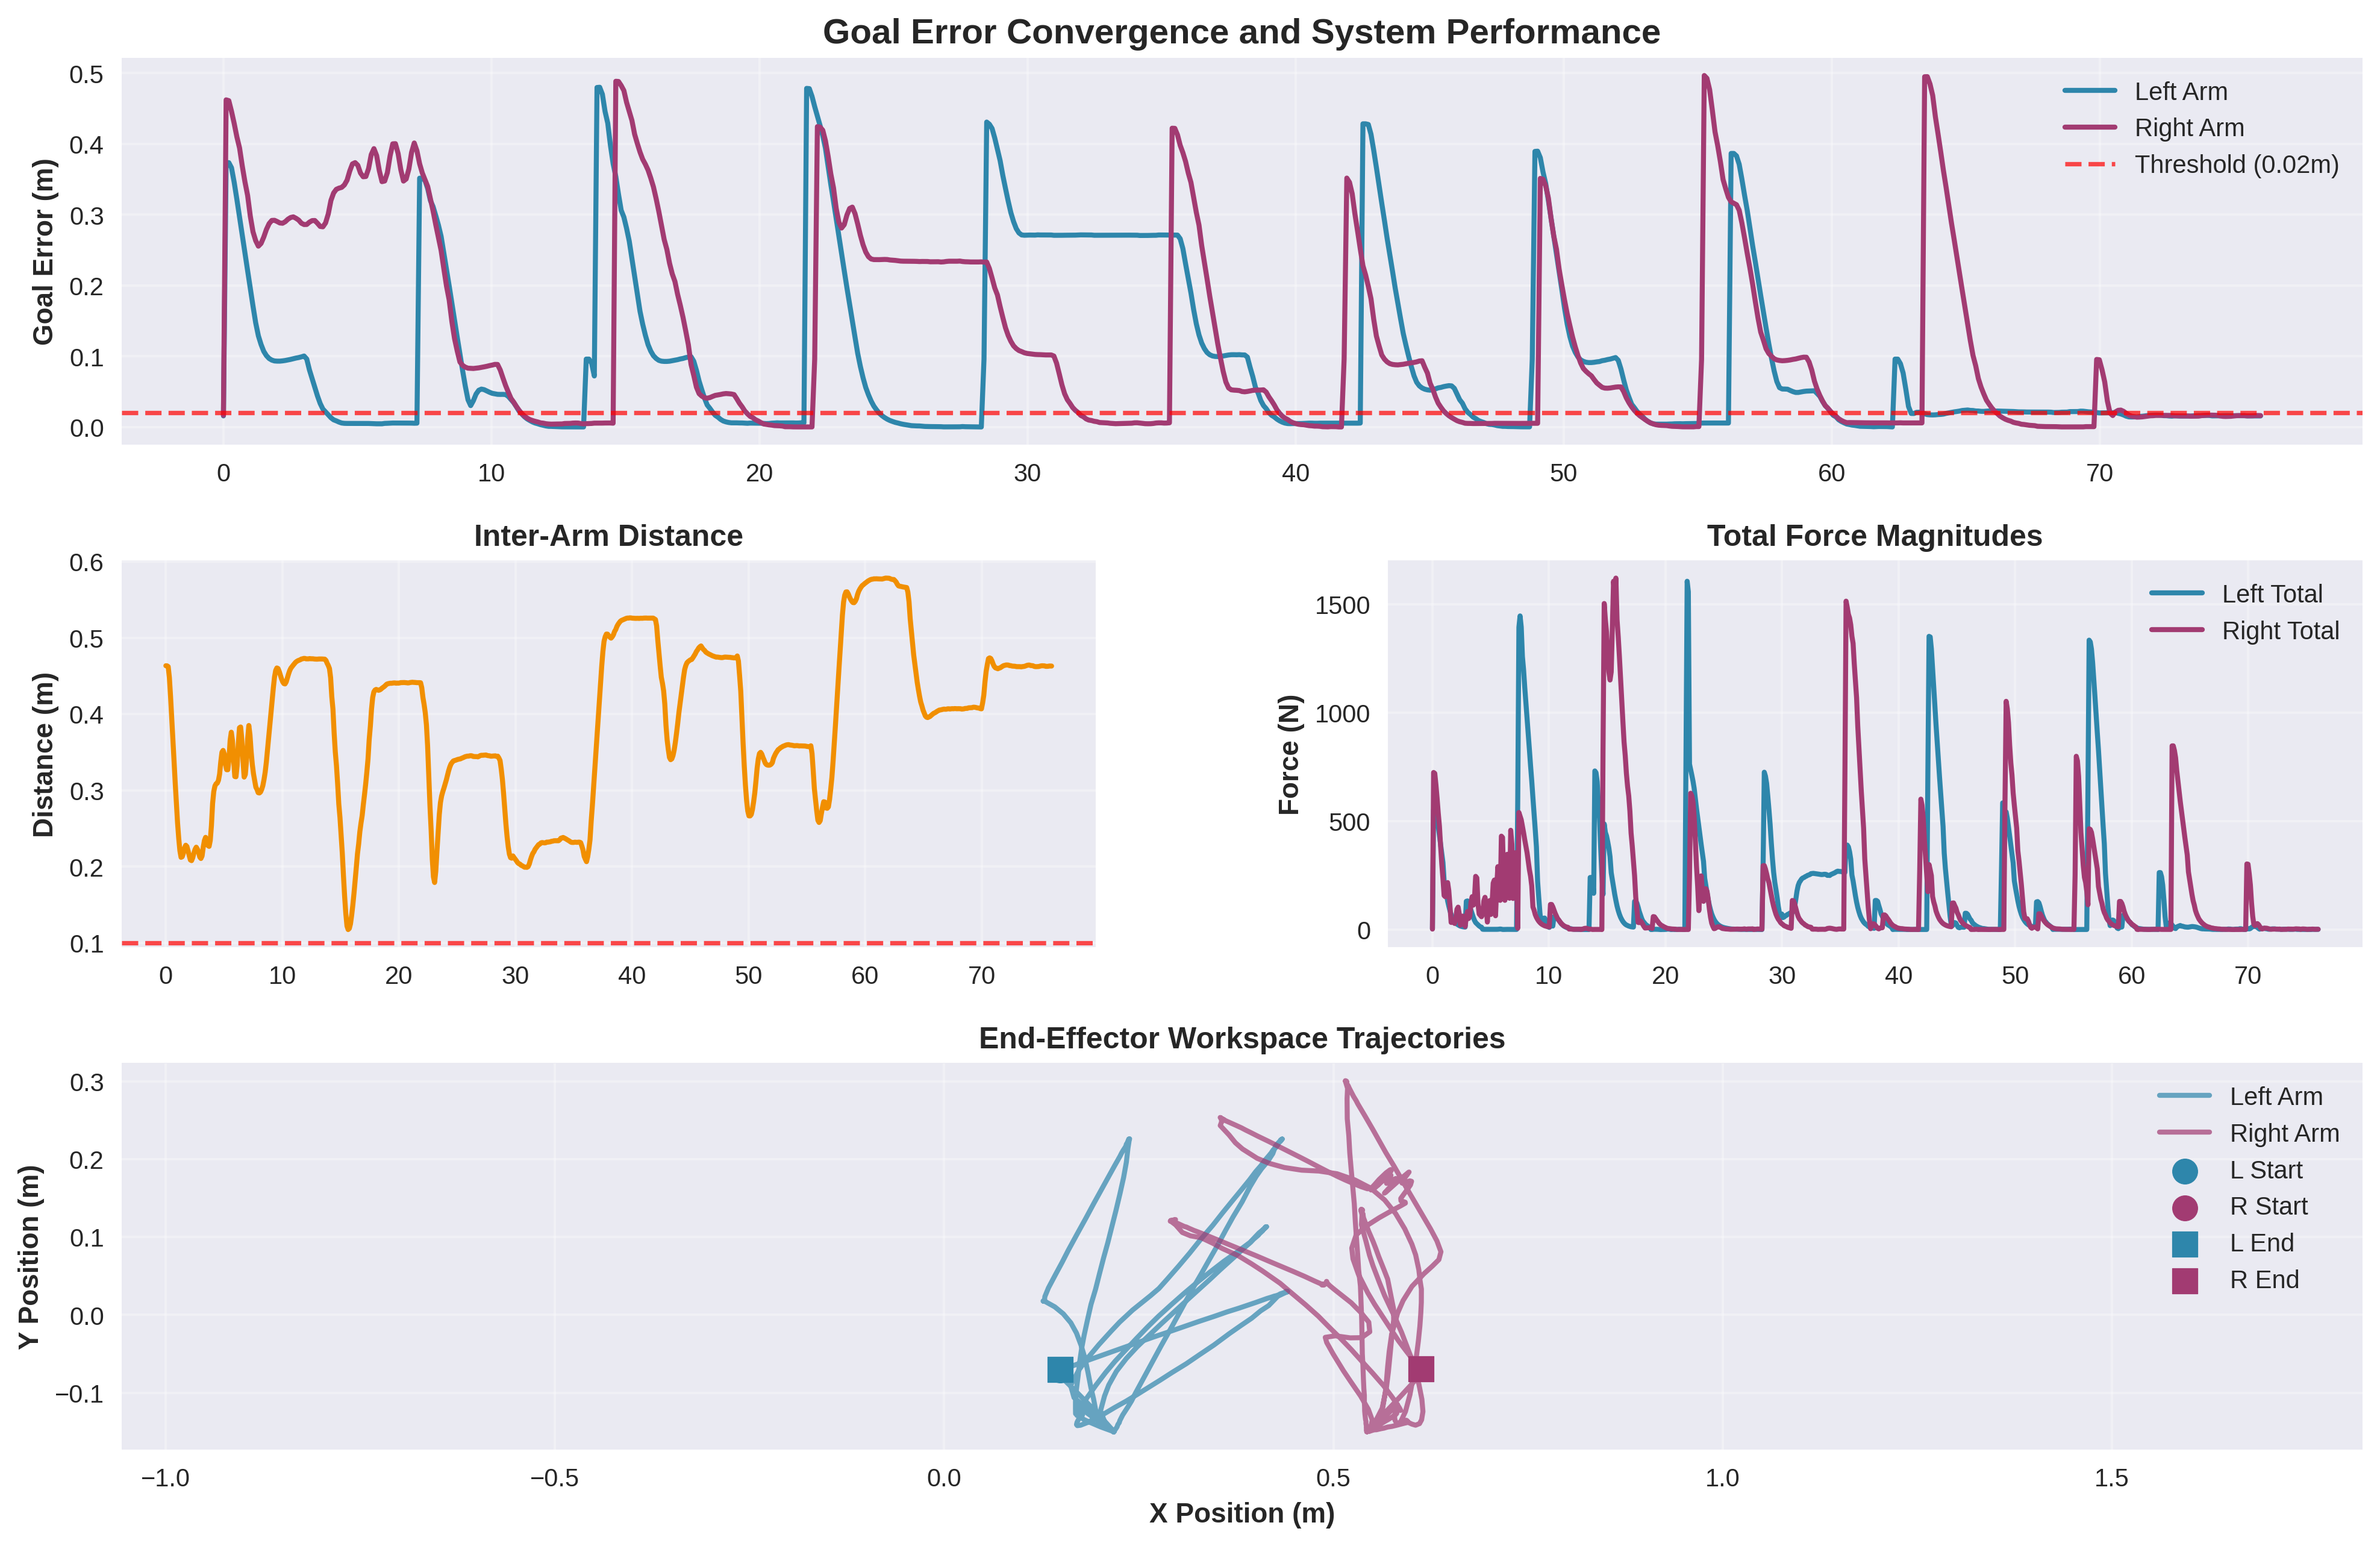
\includegraphics[width=0.75\linewidth]{Images/iapfAllocation/fixed_mixed_analysis.png}
\caption{Combined dual-arm system analysis, original fixed task allocation, mixed
objects~\citep{sk2025competitive}.}
\label{fig:cta_fixedmixed}
\end{figure}

Figure~\ref{fig:cta_dynmixed} and Figure~\ref{fig:cta_fixedmixed} show the smoother,
oscillation-free motion profile the competitive method achieves relative to the fixed allocation's
workspace conflicts, and Figure~\ref{fig:cta_seqconflict} and Figure~\ref{fig:cta_sortseq} show the
mechanism handling a compact, near-goal conflict and a complete sorting run without any collision
event, under the same iAPF controller and priority-lock switching validated in
Chapter~\ref{chap:iapf}. The temporal window's modest time overhead in the mixed-object case,
$\approx 11\%$ relative to the original fixed allocation's best-case (partial-coverage) time, is
offset by universal object handling and the larger safety margins the iAPF controller provides
throughout.

Together, Chapters~\ref{chap:distance} through~\ref{chap:task_allocation} address gaps G3, G4, and
G5 as a coherent progression rather than three independent contributions: Chapter~\ref{chap:distance}
supplies the continuous, sensor-free distance signal; Chapter~\ref{chap:iapf} establishes a stable,
empirically validated motion-planning controller under the simplifying assumption of a fixed
object-to-arm convention; and this chapter removes exactly that assumption, replacing it with
runtime competitive allocation while carrying the stable behaviour validated in
Section~\ref{sec:iapf_validation} forward unchanged. Chapter~\ref{chap:learned_control} turns from
this reactive, analytically defined controller to learning-based control, addressing gaps G6 and G7
for continuous trajectory tracking on a non-spherical wrist and for sample-efficient dual-arm
coordination learning, respectively.
